\documentclass[11pt,a4paper]{article}

% -----------------------------------------------------------------------------
% Engine and language: compile with XeLaTeX.
% -----------------------------------------------------------------------------
\usepackage{fontspec}
\usepackage{polyglossia}
\setdefaultlanguage{chinese}
\setotherlanguage{english}
\setmainfont{Noto Serif CJK SC}[
  ItalicFont={Noto Serif CJK SC},
  ItalicFeatures={FakeSlant=0.16}
]
\setsansfont{Noto Sans CJK SC}
\setmonofont{Noto Sans Mono CJK SC}[Scale=0.88]
\newfontfamily\chinesefont{Noto Serif CJK SC}[
  ItalicFont={Noto Serif CJK SC},
  ItalicFeatures={FakeSlant=0.16}
]
\newfontfamily\chinesefontsf{Noto Sans CJK SC}
\newfontfamily\chinesefonttt{Noto Sans Mono CJK SC}[Scale=0.88]
\XeTeXlinebreaklocale "zh"
\XeTeXlinebreakskip=0pt plus 1pt

% -----------------------------------------------------------------------------
% Page geometry, mathematics, tables, figures, references, and navigation.
% -----------------------------------------------------------------------------
\usepackage[left=22mm,right=22mm,top=20mm,bottom=22mm,headheight=15pt]{geometry}
\usepackage{amsmath,amssymb,mathtools}
\usepackage{graphicx}
\usepackage{booktabs}
\usepackage{xltabular}
\usepackage{array}
\usepackage{ragged2e}
\usepackage[table,dvipsnames]{xcolor}
\usepackage{enumitem}
\usepackage[numbers,sort&compress]{natbib}
\usepackage{hyperref}
\usepackage{bookmark}
\usepackage{caption}
\usepackage{fancyhdr}
\usepackage{titlesec}
\usepackage[most]{tcolorbox}
\usepackage{fvextra}
\usepackage{placeins}
\usepackage{needspace}
\usepackage{float}
\usepackage{url}

\definecolor{auditnavy}{HTML}{16324F}
\definecolor{auditblue}{HTML}{0072B2}
\definecolor{auditcyan}{HTML}{56B4E9}
\definecolor{auditteal}{HTML}{009E73}
\definecolor{auditamber}{HTML}{E69F00}
\definecolor{auditred}{HTML}{B2182B}
\definecolor{auditgray}{HTML}{5B6573}

\graphicspath{{figures/}{../figures/}}
\setlength{\parindent}{2em}
\setlength{\parskip}{0.35em}
\setlength{\tabcolsep}{4pt}
\renewcommand{\arraystretch}{1.12}
\setlist{nosep,leftmargin=2.25em,topsep=0.35em}
\setcounter{secnumdepth}{3}
\setcounter{tocdepth}{2}
\emergencystretch=2em
\Urlmuskip=0mu plus 1mu\relax

\titleformat{\section}
  {\Large\bfseries\sffamily\color{auditnavy}}
  {\thesection}{0.75em}{}
  [\vspace{0.2em}\color{auditblue}\titlerule]
\titleformat{\subsection}
  {\large\bfseries\sffamily\color{auditnavy}}
  {\thesubsection}{0.65em}{}
\titleformat{\subsubsection}
  {\normalsize\bfseries\sffamily\color{auditgray}}
  {\thesubsubsection}{0.6em}{}
\titlespacing*{\section}{0pt}{2.2ex plus 0.8ex minus 0.2ex}{1.2ex}
\titlespacing*{\subsection}{0pt}{1.8ex plus 0.5ex minus 0.2ex}{0.8ex}

\captionsetup{
  font=small,
  labelfont={bf,color=auditnavy},
  labelsep=quad,
  justification=justified,
  singlelinecheck=false,
  skip=6pt
}

\newtcolorbox{evidencebox}{
  enhanced,
  breakable,
  colback=auditblue!4,
  colframe=auditblue!55,
  boxrule=0.6pt,
  arc=1mm,
  left=2mm,right=2mm,top=1.5mm,bottom=1.5mm
}

\DefineVerbatimEnvironment{ReportVerbatim}{Verbatim}{
  fontsize=\small,
  breaklines=true,
  breakanywhere=true,
  frame=single,
  framesep=2mm,
  rulecolor=\color{auditgray!40}
}

\renewcommand{\contentsname}{目录}
\renewcommand{\listfigurename}{图目录}
\renewcommand{\listtablename}{表目录}
\renewcommand{\figurename}{图}
\renewcommand{\tablename}{表}
\renewcommand{\refname}{参考文献}

\hypersetup{
  unicode=true,
  colorlinks=true,
  linkcolor=auditnavy,
  citecolor=auditteal,
  urlcolor=auditblue,
  pdftitle={J-TEXT 至 EAST 小样本迁移与因果在线主动适配技术报告},
  pdfauthor={J-TEXT--EAST Project},
  pdfsubject={可审计的跨装置破裂预警研究与复现说明},
  pdfkeywords={tokamak, disruption prediction, transfer learning, online adaptation}
}

\pagestyle{fancy}
\fancyhf{}
\fancyhead[L]{\small\sffamily J-TEXT 至 EAST 破裂预警研究}
\fancyhead[R]{\small\sffamily JTE-XFER-OA-TR-02 · v3.0}
\fancyfoot[C]{\small\thepage}
\renewcommand{\headrulewidth}{0.35pt}
\renewcommand{\footrulewidth}{0pt}
\fancypagestyle{plain}{
  \fancyhf{}
  \fancyfoot[C]{\small\thepage}
  \renewcommand{\headrulewidth}{0pt}
}

\begin{document}
\hypersetup{pageanchor=false}

\begin{titlepage}
  \thispagestyle{empty}
  \begin{flushright}
    {\small\sffamily\color{auditgray}技术报告编号：JTE-XFER-OA-TR-02\par}
    {\small\sffamily\color{auditgray}版本：3.0 · 2026年8月23日\par}
  \end{flushright}

  \vspace*{18mm}
  \noindent{\color{auditblue}\rule{\textwidth}{2.2pt}}\par
  \vspace{8mm}
  {\Huge\bfseries\sffamily\color{auditnavy}
    J-TEXT 至 EAST 小样本迁移与\par
    因果在线主动适配技术报告\par}
  \vspace{4mm}
  {\Large\sffamily\color{auditgray}
    数据合同、模型方法、消融验证与证据边界\par}
  \vspace{7mm}
  \noindent{\color{auditblue}\rule{\textwidth}{0.7pt}}\par

  \vfill
  \noindent\begin{tabularx}{\textwidth}{@{}>{\bfseries\sffamily\color{auditnavy}}p{34mm}X@{}}
    文档用途 & 面向导师、同行评审与相关技术部门的正式研究底稿及复现说明 \\
    研究主线 & J-TEXT 源模型 $\rightarrow$ EAST 110炮适配 $\rightarrow$ EAST 360炮因果在线回放 \\
    标签权威源 & HDF5 中的结局、DownTime 与信号内容；历史炮表不得覆盖 HDF5 标签 \\
    正式执行环境 & \texttt{rl\_env}，NVIDIA GeForce RTX 5070；单 GPU 因果执行 \\
    证据状态 & \texttt{DEVELOPMENT\_EVIDENCE\_NOT\_}\allowbreak{}\texttt{INDEPENDENT\_CONFIRMATION} \\
    数据发布边界 & 原始 HDF5 不进入 Git 仓库；通过内容清单和 SHA256 绑定外部数据 \\
  \end{tabularx}

  \vspace{12mm}
  \begin{evidencebox}
    \textbf{证据声明。} 本报告中的 TEST220、support110 和 balanced360 均参与了不同程度的方法开发、模型选择或阈值选择。全部主结果因此属于可审计的开发性实验依据，不得解释为独立未来流确认或装置部署验收结果。
  \end{evidencebox}

  \vfill
  {\small\sffamily\color{auditgray}
    仓库交付包含标准 XeLaTeX 工程、机器可读证据、逐炮账本、确定性统计图和概念方法图。\par}
\end{titlepage}

\hypersetup{pageanchor=true}
\pagenumbering{roman}
\section*{摘要}
\addcontentsline{toc}{section}{摘要}
本报告系统说明 J-TEXT 至 EAST 破裂预警链路的研究目标、数据与标签合同、跨装置共享/私有特征分解、小样本迁移、炮内无标签个性化、炮间主动查询与监督更新，以及相应消融和负对照。统一三随机种子谱系的开发性结果为：J-TEXT TEST220 的 operational TPR（提前量大于10 ms）为0.8515、FPR为0.2121、AUC为0.9219；EAST balanced360 静态迁移的 TPR（提前量不小于30 ms）为0.8407、FPR为0.1667；同一父模型的因果在线回放对应为0.8481和0.1519。在线阶段在当前开发流上降低了误报，同时保持灵敏度，但中位提前量未显示稳定改善。

上述结果不等价于独立验证：balanced360 曾参与方法逆向分析和候选筛选，support110 同时用于目标适配与阈值选择，源域仍存在已经识别但尚未与现有目标策略兼容的 padding shortcut。报告因此把“链路已贯通”“开发性增益存在”与“尚未完成未来流确认”明确分开，并给出能够升级证据等级的冻结式前瞻验证方案。

\noindent\textbf{关键词：} 托卡马克；破裂预警；小样本迁移；测试时适配；在线主动学习；因果评估；证据审计

\begin{figure}[htbp]
  \centering
  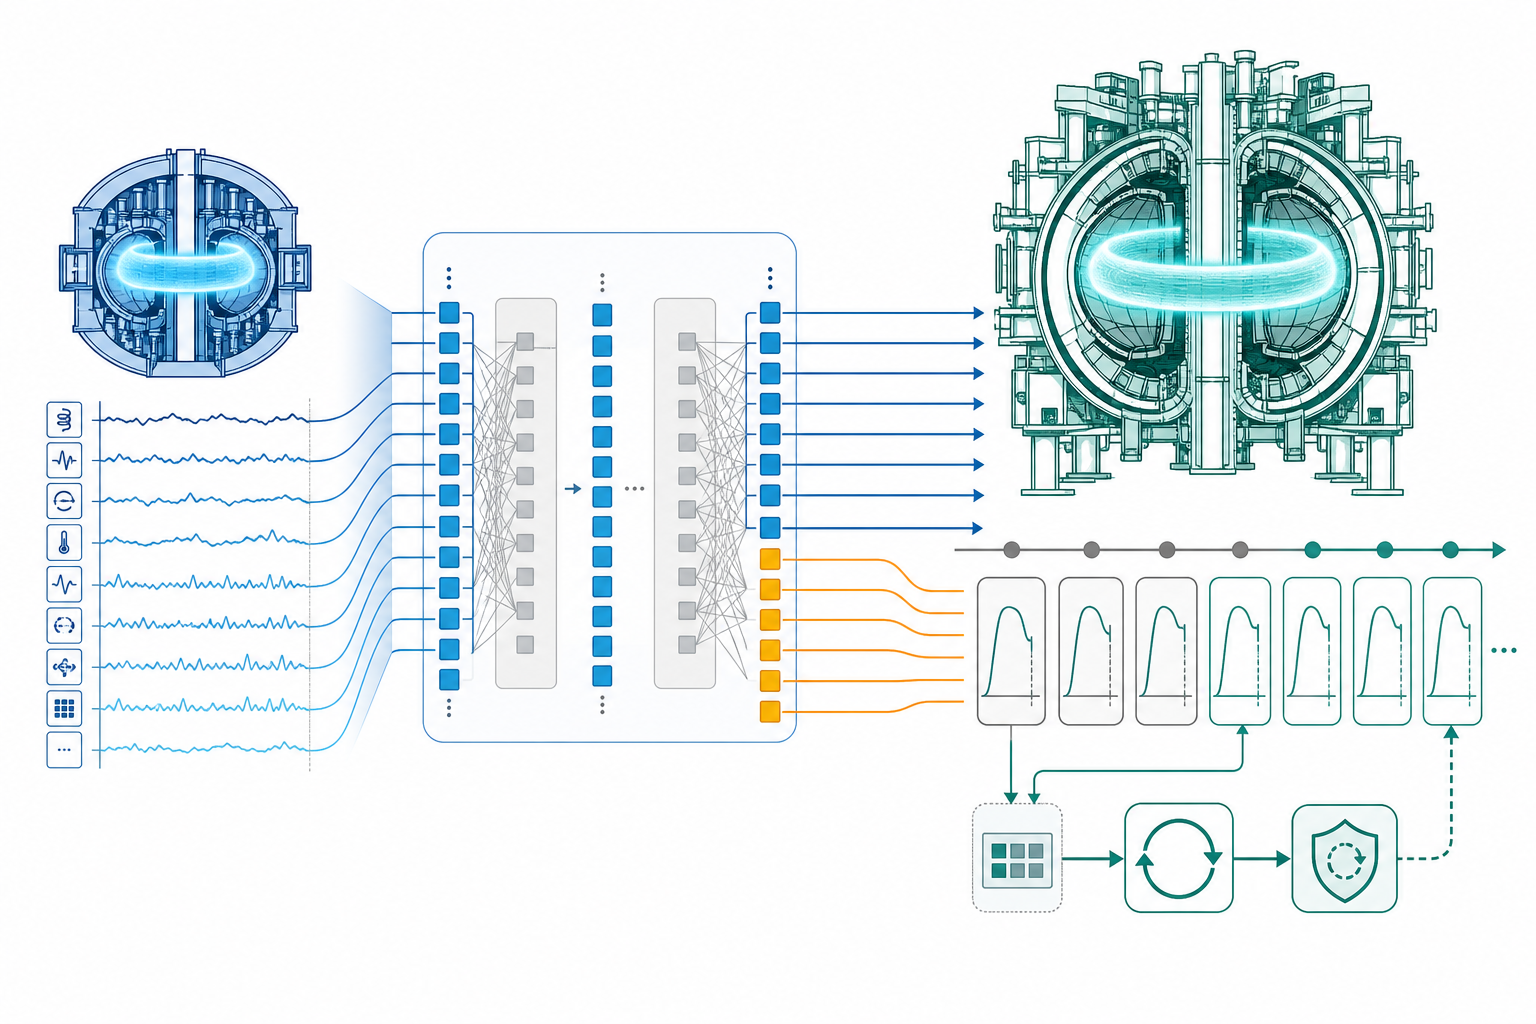
\includegraphics[width=0.80\textwidth]{concept_graphical_abstract_v1.png}
  \caption{J-TEXT 源表示、共享/目标私有迁移和 EAST 因果在线适配的图形摘要。该图由生成式图像工具制作，仅表达方法结构，不包含测量数据、模型输出或实验数值。}
  \label{fig:graphical-abstract}
\end{figure}

\clearpage
\tableofcontents
\clearpage
\listoffigures
\clearpage

\pagenumbering{arabic}
% Generated from TECHNICAL_REPORT_zh.md. Do not edit manually.
% Regenerate with scripts/convert_technical_report_zh_to_latex.py.


\FloatBarrier
\section*{文档使用说明}
\addcontentsline{toc}{section}{文档使用说明}
本报告分为三个层次：第1至17节给出研究问题、数据合同、工程方法、主要结果、消融实验和证据成熟度；第18至30节给出数学定义、损失函数、状态更新和完整因果算法；第31至35节给出符号索引、代码与证据映射、复现程序、综合技术结论和参考文献。读者可先阅读第1、3、6、7、8、14和16节掌握结论，再查阅后续公式与实现细节。

术语约定如下：首次出现时使用中文名称并附英文术语；后文保留行业通用缩写。\texttt{support110}\allowbreak{}、\texttt{TEST220}\allowbreak{}、\texttt{balanced360}\allowbreak{} 均为冻结数据角色名称，而非性能等级。本文中的“在线”是按炮号顺序的历史因果回放，不表示已经接入装置控制系统。


\subsection*{证据等级}

{\small
\renewcommand{\arraystretch}{1.18}
\begin{xltabular}{\textwidth}{@{}>{\RaggedRight\arraybackslash}X>{\RaggedRight\arraybackslash}X>{\RaggedRight\arraybackslash}X@{}}
\toprule
\rowcolor{auditblue!10}
等级 & 定义 & 本报告中的典型内容 \\
\midrule
\endfirsthead
\toprule
\rowcolor{auditblue!10}
等级 & 定义 & 本报告中的典型内容 \\
\midrule
\endhead
E0：合同证据 & 数据角色、标签权威源、信息访问边界和评价公式 & HDF5 标签合同、lead 定义、\texttt{predict \ensuremath{\rightarrow} seal \ensuremath{\rightarrow} reveal \ensuremath{\rightarrow} update}\allowbreak{} 顺序 \\
E1：执行证据 & 可由代码、配置、哈希、逐炮账本或自动验证器复核的事实 & checkpoint 血缘、炮表 SHA256、逐炮预测、参数更新回执 \\
E2：开发性实验依据 & 在参与方法开发的数据上获得的比较结果 & TEST220、support110 与 balanced360 上的主结果和消融 \\
E3：独立确认依据 & 方法、阈值和停止规则冻结后，在未参与开发的新时序流上一次性获得的结果 & \textbf{本项目尚未完成} \\
\bottomrule
\end{xltabular}
}

除非另有说明，本报告的性能结论均属于 E2；代码可执行性、标签访问顺序和文件哈希等审计结论属于 E1。任何 E2 结果均不得在未补充 E3 验证的情况下解释为部署性能。


\subsection*{主要缩略语与数据角色}

{\small
\renewcommand{\arraystretch}{1.18}
\begin{xltabular}{\textwidth}{@{}>{\RaggedRight\arraybackslash}X>{\RaggedRight\arraybackslash}X@{}}
\toprule
\rowcolor{auditblue!10}
术语 & 定义 \\
\midrule
\endfirsthead
\toprule
\rowcolor{auditblue!10}
术语 & 定义 \\
\midrule
\endhead
TPR /\allowbreak{} FPR & 真阳性率 /\allowbreak{} 假阳性率；TPR 按规定最低提前量计算 \\
TTD & Time to disruption，当前因果端点距破裂时刻的剩余时间 \\
TEST220 & J-TEXT 的220炮平衡比较集；在同次执行中锁定后读取，但并非严格时序未来集 \\
support110 & EAST 的110炮小样本支持集；用于目标适配和目标阈值选择 \\
balanced360 & EAST 的180破裂/\allowbreak{}180安全炮顺序开发流；用于静态比较和因果在线回放 \\
PADFIX & 针对有效历史长度/\allowbreak{}左填充捷径的上下文一致性与条件对抗训练 \\
shared17 /\allowbreak{} private8 & 17维跨装置共享输入与8维 EAST 私有输入的结构化分解 \\
static /\allowbreak{} online & 冻结迁移模型的一次性预测 /\allowbreak{} 按炮号顺序执行的因果在线适配 \\
\bottomrule
\end{xltabular}
}


\FloatBarrier
\section{报告摘要与主要结论}

\begin{figure}[htbp]
  \centering
  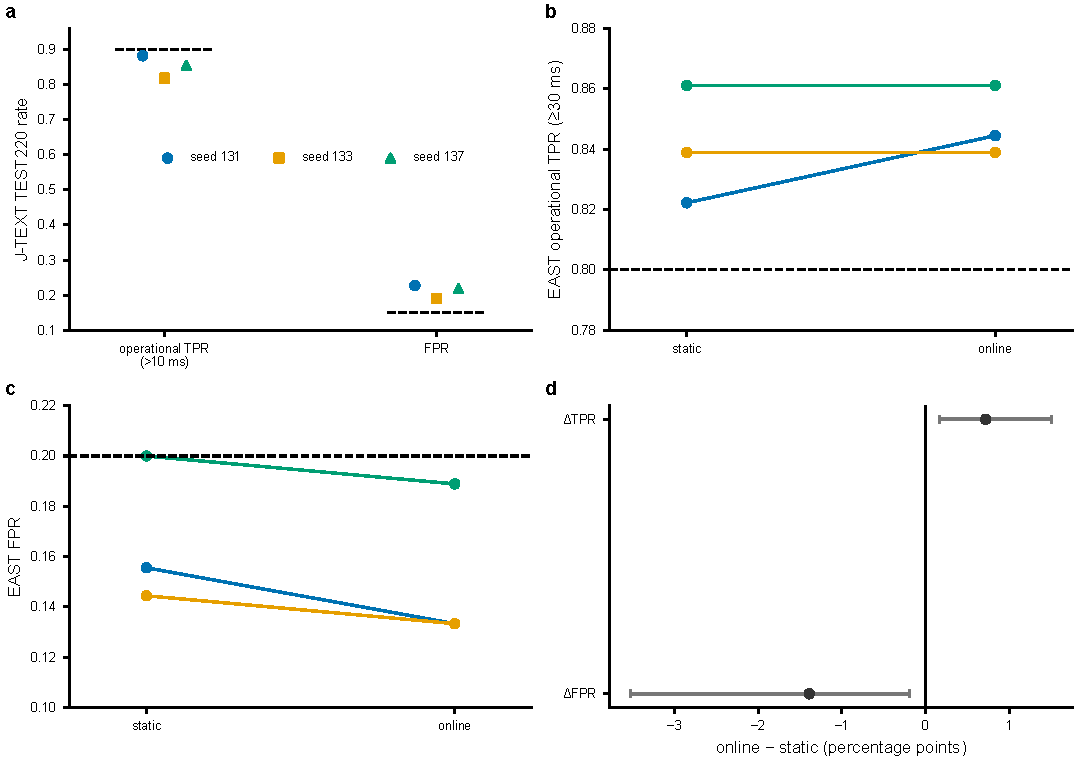
\includegraphics[width=\linewidth]{fig2_same_lineage_metrics_and_block_resampling.pdf}
  \caption{同一模型谱系下的三阶段指标与静态至在线的配对变化。所有数值均由冻结逐炮账本重算；重采样区间仅用于开发流描述，不构成独立确认。}
  \label{fig:three-stage-metrics}
\end{figure}

\subsection{研究目标}
本项目研究在 EAST 标注样本受限条件下，如何将 J-TEXT 上学习得到的破裂风险表示迁移至 EAST，并通过严格遵守时间顺序的信息访问协议实施炮内无标签适配和炮间主动监督更新。炮内适配借鉴测试时自适配与持续测试时适配的基本思想\citep{wang2021tent,niu2022eata,wang2022cotta}，炮间查询和更新则与在线持续适配研究的问题设置相关\citep{zhou2022online}；本项目在此基础上增加了标签访问封存、双时间尺度参数、物理矛盾伪监督和原子回滚。完整计算链路保持统一模型谱系：


\begin{ReportVerbatim}
J-TEXT TRAIN1353 训练 causal Patch Transformer
→ VAL160 选择 epoch 与源域阈值
→ 在同次运行内锁定后评估 count-aligned TEST220 比较集
→ 同 seed checkpoint 在 EAST 固定110炮上做小样本迁移
→ 完整静态预测并封存 EAST balanced360
→ 重置到相同迁移父模型
→ 按炮号走完360炮在线主动流
→ predict → seal → query → selected HDF5 reveal → later-shot update
\end{ReportVerbatim}

各阶段均由相同 seed 的源模型、目标适配器和在线父模型衔接，避免使用彼此无关的 checkpoint 拼接结果。三阶段核心指标如下。


{\scriptsize
\renewcommand{\arraystretch}{1.18}
\begin{xltabular}{\textwidth}{@{}>{\RaggedRight\arraybackslash}X>{\RaggedRight\arraybackslash}X>{\RaggedRight\arraybackslash}X>{\RaggedRight\arraybackslash}X>{\RaggedRight\arraybackslash}X>{\RaggedRight\arraybackslash}X@{}}
\toprule
\rowcolor{auditblue!10}
阶段 & 正式评估口径 & operational TPR & FPR & AUC & operational median lead \\
\midrule
\endfirsthead
\toprule
\rowcolor{auditblue!10}
阶段 & 正式评估口径 & operational TPR & FPR & AUC & operational median lead \\
\midrule
\endhead
J-TEXT 源模型 & TEST220，lead > 10 ms & \textbf{0.8515} & \textbf{0.2121} & \textbf{0.9219} & \textbf{116.6 ms} \\
J-TEXT 至 EAST 静态迁移 & balanced360，lead \ensuremath{\geq} 30 ms & \textbf{0.8407} & \textbf{0.1667} & 未归档统一连续分数 & \textbf{242.0 ms} \\
EAST 因果在线适配 & 同一 balanced360 顺序流，lead \ensuremath{\geq} 30 ms & \textbf{0.8481} & \textbf{0.1519} & 未归档统一连续分数 & \textbf{229.5 ms} \\
\bottomrule
\end{xltabular}
}

严格 EAST-only 基线仅使用 support110，随机初始化完整17维 Transformer，并拟合 EAST 本地稳健缩放器。三个 seed 的均值为 \texttt{TPR@30=0.7963}\allowbreak{}、\texttt{FPR=0.1444}\allowbreak{}、\texttt{J=0.6519}\allowbreak{}、\texttt{median lead=165.6 ms}\allowbreak{}。静态迁移相对该基线的 TPR 增加0.0444、FPR增加0.0222，综合指标 $J=TPR_{30}-FPR$ 增加0.0222，中位提前量增加约76.5 ms。仅复用 J-TEXT 缩放器而不继承源模型权重的随机模型为 \texttt{TPR@30=0.7315}\allowbreak{}、\texttt{FPR=0.1056}\allowbreak{}，表明缩放统计本身不足以构成有效迁移。由于 EAST-only 更新完整编码器，而迁移模型只更新受限目标路径，两者不构成严格的等参数量或等计算量比较。


\subsection{在线适配的配对变化}
在线相对静态的三 seed 配对圆形 moving-block 重采样（block=20，5,000 次）得到：


\begin{itemize}
\item FPR 变化中位数 \texttt{-}\allowbreak{}\texttt{0}\texttt{.}\allowbreak{}\texttt{01389}\allowbreak{}，95\% 描述区间 \texttt{[-0.03521, -0.00193]}\allowbreak{}；
\item operational TPR@30 ms 变化 \texttt{+}\allowbreak{}\texttt{0}\texttt{.}\allowbreak{}\texttt{00717}\allowbreak{}，95\% 描述区间 \texttt{[+0.00171, +0.01500]}\allowbreak{}；
\item operational median lead 变化 \texttt{-11.66 ms}\allowbreak{}，95\% 描述区间 \texttt{[-69.01, +4.00] ms}\allowbreak{}。
\end{itemize}

block size 10、20、30和45的方向一致。然而，该重采样没有在每一条重构历史上重新执行在线学习，且 balanced360 已用于972个 episode 候选筛选。因此上述区间仅用于描述冻结开发账本上的局部稳定性，不是面向未来数据的选择后置信区间。中位提前量未显示稳定改善。


\subsection{关键技术发现与限制}
审计同时识别出源模型的上下文长度捷径：隐藏表示预测窗口有效历史长度的 probe AUC 为 \texttt{0}\texttt{.}\allowbreak{}\texttt{955}\texttt{/\allowbreak{}}\allowbreak{}\texttt{0}\texttt{.}\allowbreak{}\texttt{929}\texttt{/\allowbreak{}}\allowbreak{}\texttt{0}\texttt{.}\allowbreak{}\texttt{937}\allowbreak{}，高于预注册门槛0.65。PADFIX 将该指标降至 \texttt{0}\texttt{.}\allowbreak{}\texttt{624}\texttt{/\allowbreak{}}\allowbreak{}\texttt{0}\texttt{.}\allowbreak{}\texttt{645}\texttt{/\allowbreak{}}\allowbreak{}\texttt{0}\texttt{.}\allowbreak{}\texttt{649}\allowbreak{}，但源域及时灵敏度下降；将既有在线策略直接迁移至 PADFIX 父模型后，三个 seed 的 FPR 均上升。因此，当前结果支持“工程链路可执行且具有开发性增益”，但不足以支持“已识别全部破裂机理”或“达到装置部署验收条件”等更强结论。


\FloatBarrier
\section{数据合同与标签依据}

\begin{figure}[htbp]
  \centering
  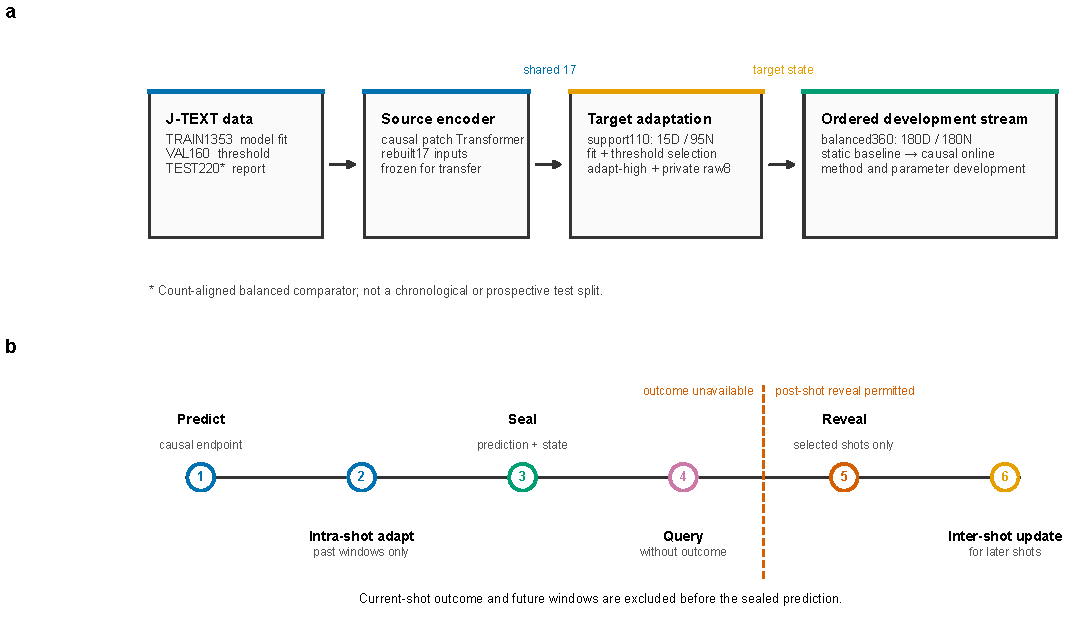
\includegraphics[width=\linewidth]{fig1_protocol_and_causal_contract.pdf}
  \caption{数据角色、标签权威源和在线信息访问顺序。当前炮必须先完成预测与封存，随后才允许作出查询并揭示被选炮标签。}
  \label{fig:data-contract}
\end{figure}

\subsection{J-TEXT}
HDF5 总计 1,733 炮：378 破裂、1,355 安全。正式源域划分为：


{\footnotesize
\renewcommand{\arraystretch}{1.18}
\begin{xltabular}{\textwidth}{@{}>{\RaggedRight\arraybackslash}X>{\RaggedRight\arraybackslash}X>{\RaggedRight\arraybackslash}X>{\RaggedRight\arraybackslash}X>{\RaggedRight\arraybackslash}X@{}}
\toprule
\rowcolor{auditblue!10}
角色 & 总数 & 破裂 & 安全 & 用途 \\
\midrule
\endfirsthead
\toprule
\rowcolor{auditblue!10}
角色 & 总数 & 破裂 & 安全 & 用途 \\
\midrule
\endhead
TRAIN1353 & 1,353 & 188 & 1,165 & 源模型与 scaler 拟合 \\
VAL160 & 160 & 80 & 80 & epoch 和阈值选择 \\
TEST220 & 220 & 110 & 110 & 同次执行内锁定后比较评估 \\
\bottomrule
\end{xltabular}
}

三者炮号零重叠，但不是严格时间块。每个文件只是为稳定序列化按炮号排序；TRAIN/\allowbreak{}VAL/\allowbreak{}TEST 的炮号范围相互穿插。它们是固定 \texttt{paper131}\texttt{-}\allowbreak{}\texttt{count}\texttt{-}\allowbreak{}\texttt{aligned}\allowbreak{} 比较队列，VAL160/\allowbreak{}TEST220 又是结果平衡集，不模拟真实源域患病率或未来部署流。三个 roster SHA256 分别为：


\begin{ReportVerbatim}
TRAIN1353 ad403f388694e2dc2b8855dae9d084c319243bd02bdf465abe743919a1b4f9d4
VAL160   bf726a031953c6d0aceba04e10b02b713ecca70a32e27077cca372e45ee9d2be
TEST220  b963c2973c198a833e44017f73e0a11749d50d7144f5758b0ec9bfcd7763868e
\end{ReportVerbatim}


\subsection{EAST}
EAST HDF5 总计 2,953 炮：1,198 破裂、1,755 安全。


\begin{itemize}
\item 迁移支持集固定为 110 炮；历史 JSON 标题分组是 10D/\allowbreak{}100N，但 HDF5 真标签重算后为 \textbf{15D/\allowbreak{}95N}。
\item balanced360 为 \textbf{180D/\allowbreak{}180N}，按炮号顺序执行，与 support110 零重叠。
\item balanced360 manifest SHA256：
\end{itemize}


\begin{ReportVerbatim}
657cab542bd987f9c97c3cb88867a9cc828373b32e6ee58d450451461c6ec825
\end{ReportVerbatim}

历史清单仅用于记录候选炮号来源；实验标签、指标及时间锚点均以 HDF5 为准。证据生成器同时保留“历史分组10/\allowbreak{}100”和“HDF5权威分组15/\allowbreak{}95”，以支持标签谱系审计并防止混用。


\FloatBarrier
\section{跨装置迁移的主要技术障碍}

\begin{figure}[htbp]
  \centering
  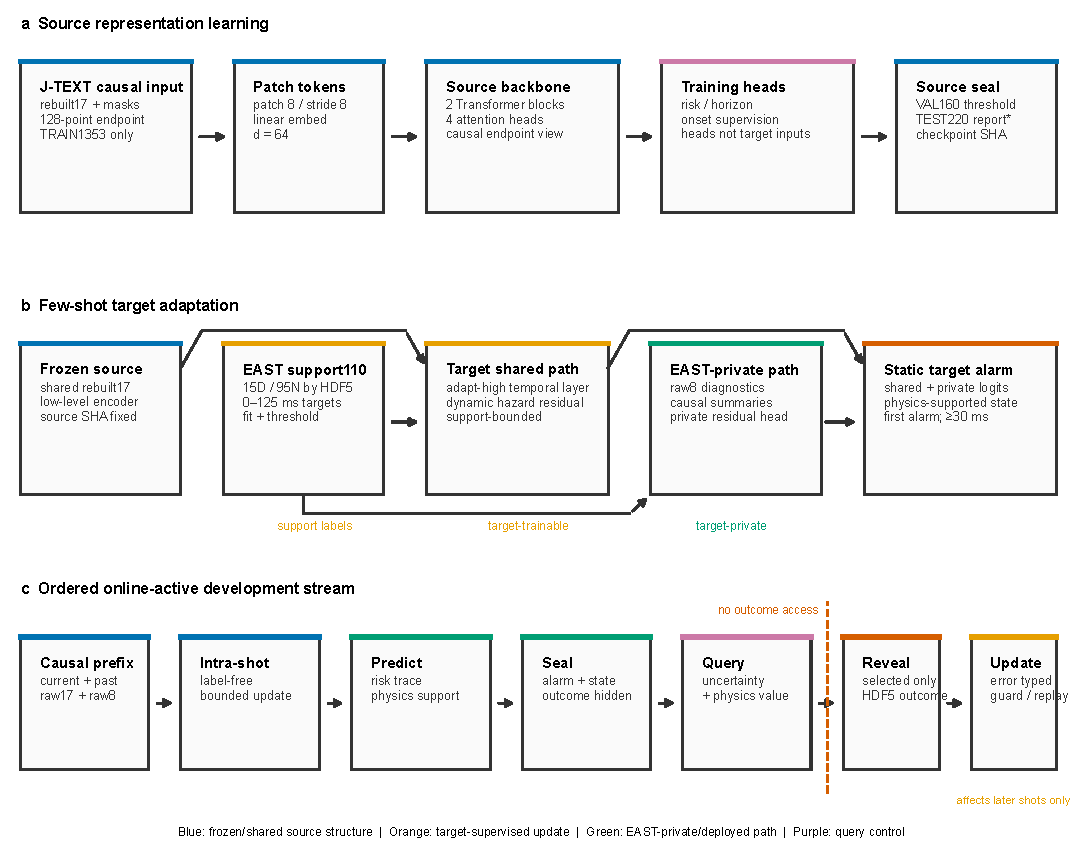
\includegraphics[width=\linewidth]{fig0_end_to_end_model_architecture.pdf}
  \caption{实际执行的源域监督、目标域小样本适配、EAST 私有支路与因果在线更新结构。颜色表示计算角色，不表示证据等级。}
  \label{fig:architecture}
\end{figure}
历史迁移实验的性能不足主要由以下三类结构性混杂共同造成，而非单一损失权重设置所致。该判断与既有跨托卡马克迁移研究关于“局部物理特征较易共享、上层时间动力学需要目标域适配”的观察一致\citep{zheng2023transfer,shen2023pgfeda,shen2024thesis,zheng2025phydanet}，同时遵循域适配可识别性限制：当类别先验、观测函数和标签条件分布同时变化时，降低边缘域距离并不保证目标任务风险下降\citep{ganin2016dann,sun2016coral,bendavid2010impossibility}。


\begin{enumerate}
\item \textbf{23 维名义同名不等于物理同构。} CIII、MNM、Mirnov 幅值、\texttt{ne}\texttt{\_}\allowbreak{}\texttt{nG}\allowbreak{}、\texttt{qa}\texttt{\_}\allowbreak{}\texttt{proxy}\allowbreak{}、SXR 均值、XUV ratio 等通道在单位、可用性、探针实现或构造方法上不稳定。直接 DANN/\allowbreak{}MMD/\allowbreak{}CORAL 会把装置差异、缺失模式和类别比例一起“对齐”。
\item \textbf{上层时间动力学并不共享。} J-TEXT 炮短，EAST 炮长；两者破裂演化速度和采样上下文分布不同。强制共享完整上层时间读出会造成负迁移。
\item \textbf{源域 padding 成为捷径。} J-TEXT 短炮和破裂窗口的左填充比例不同；即使模型整体指标不差，它也可能利用有效历史长度而不是仅靠物理演化。这属于典型的 shortcut learning 风险\citep{geirhos2020shortcut}。
\end{enumerate}

据此，最终方案采用结构化分解：17维可审计语义进入跨装置共享路径，剩余8维进入 EAST 私有分支；低层表示保留源域初始化，高层时间动力学和风险残差由 EAST 独立适配；在线阶段分别建模炮内更新价值、标签查询价值、揭示后监督价值和部署侧误报保护价值。


\FloatBarrier
\section{跨装置共享特征与目标私有特征}

\subsection{跨装置 shared rebuilt17}
正式共享特征为：


\begin{ReportVerbatim}
Bt, ip_A, Bt_over_Ip, Ip_diff, v_loop, Z_proxy,
sxr_kurt, sxr_skew, sxr_var,
xuv_kurt, xuv_skew, xuv_var,
Mir_avg_fre, n=1 amplitude, mode_number_n, dx_a, dy_a
\end{ReportVerbatim}

关键处理：


\begin{itemize}
\item J-TEXT \texttt{ip}\allowbreak{} 只做一次 kA\ensuremath{\rightarrow}A；
\item \texttt{Bt}\texttt{/\allowbreak{}}\allowbreak{}\texttt{Ip}\allowbreak{}、\texttt{Ip}\texttt{\_}\allowbreak{}\texttt{diff}\allowbreak{}、\texttt{Z\_\allowbreak{}proxy=v\_\allowbreak{}loop/\allowbreak{}ip}\allowbreak{} 在单位统一后重算；
\item 全零 MHD 频率/\allowbreak{}模数炮标记为 unavailable，而不是物理零；
\item scaler 由合法训练域拟合，缺失先保留 mask，再以缩放后的零作为 sentinel。
\end{itemize}


\subsection{EAST-private raw8}
以下 8 个通道不再强行跨域对齐：


\begin{ReportVerbatim}
CIII, MNM, Mir_VV, Mir_avg_amp,
ne_nG, qa_proxy, sxr_mean, xuv_ratio
\end{ReportVerbatim}

它们仍有价值，但只在 EAST 域内进入 1,089 参数的 sidecar。每通道提取最后值、均值、标准差、全窗增量、近期增量和可用率，最后层零初始化，logit 残差有界。raw8 scaler 只由 support110 拟合。


\FloatBarrier
\section{J-TEXT 源域风险模型}

\subsection{实际架构}
实际 checkpoint 合同采用 PatchTST 类时间分块表征\citep{nie2023patchtst}，具体为：


\begin{ReportVerbatim}
rebuilt17-patch-transformer-128x8-d64-l2-h4-v1
\end{ReportVerbatim}

即 128 ms 因果窗口、patch=8、stride=8、\texttt{d\_\allowbreak{}model=64}\allowbreak{}、2 层、4 头。更早计划中的 256 点没有被这一血缘实际执行，论文中已经显式记录这个偏差。

破裂窗口在 TTD \texttt{[0,125] ms}\allowbreak{} 为正；更早窗口和安全炮窗口为负。训练按炮和类别平衡采样，VAL160 在 operational TPR@>10ms\ensuremath{\geq}0.90 的候选中选择最低 FPR 阈值，TEST220 在 checkpoint 和阈值锁定后读取。这里的“锁定”只描述本次执行顺序；由于划分本身是非时序、结果平衡的 count-aligned 比较队列，不能把 TEST220 升格为真实前瞻独立集。

源域逐炮账本已补齐首次越阈的 \texttt{alarm}\texttt{\_}\allowbreak{}\texttt{endpoint}\allowbreak{} 与 \texttt{alarm}\texttt{\_}\allowbreak{}\texttt{time}\texttt{\_}\allowbreak{}\texttt{s}\allowbreak{}。证据构建器不再直接相信归档的 \texttt{lead}\texttt{\_}\allowbreak{}\texttt{ms}\allowbreak{}，而是用 \texttt{HDF5 /\allowbreak{}meta/\allowbreak{}DownTime - alarm\_\allowbreak{}time\_\allowbreak{}s}\allowbreak{} 独立重算，并以 \texttt{1e-6 ms}\allowbreak{} 容差核对；缺失 endpoint 时直接失败。三个冻结 checkpoint 在注册的确定性 PyTorch 设置下重放后，原有 score、报警决策和 lead 全部一致。


\subsection{三 seed 结果}

{\scriptsize
\renewcommand{\arraystretch}{1.18}
\begin{xltabular}{\textwidth}{@{}>{\RaggedRight\arraybackslash}X>{\RaggedRight\arraybackslash}X>{\RaggedRight\arraybackslash}X>{\RaggedRight\arraybackslash}X>{\RaggedRight\arraybackslash}X>{\RaggedRight\arraybackslash}X@{}}
\toprule
\rowcolor{auditblue!10}
seed & TP>10/\allowbreak{}FP/\allowbreak{}FN>10/\allowbreak{}TN & operational TPR >10ms & FPR & AUC & operational median lead \\
\midrule
\endfirsthead
\toprule
\rowcolor{auditblue!10}
seed & TP>10/\allowbreak{}FP/\allowbreak{}FN>10/\allowbreak{}TN & operational TPR >10ms & FPR & AUC & operational median lead \\
\midrule
\endhead
131 & 97/\allowbreak{}25/\allowbreak{}13/\allowbreak{}85 & 0.8818 & 0.2273 & 0.9307 & 107.2 ms \\
133 & 90/\allowbreak{}21/\allowbreak{}20/\allowbreak{}89 & 0.8182 & 0.1909 & 0.9253 & 120.7 ms \\
137 & 94/\allowbreak{}24/\allowbreak{}16/\allowbreak{}86 & 0.8545 & 0.2182 & 0.9098 & 122.1 ms \\
\bottomrule
\end{xltabular}
}

上述数据对应后续最佳 EAST 迁移链路实际继承的源 checkpoint。为保持模型谱系一致性，报告不得用其他源模型的指标替代该组结果。


\FloatBarrier
\section{EAST 小样本迁移}

\begin{figure}[htbp]
  \centering
  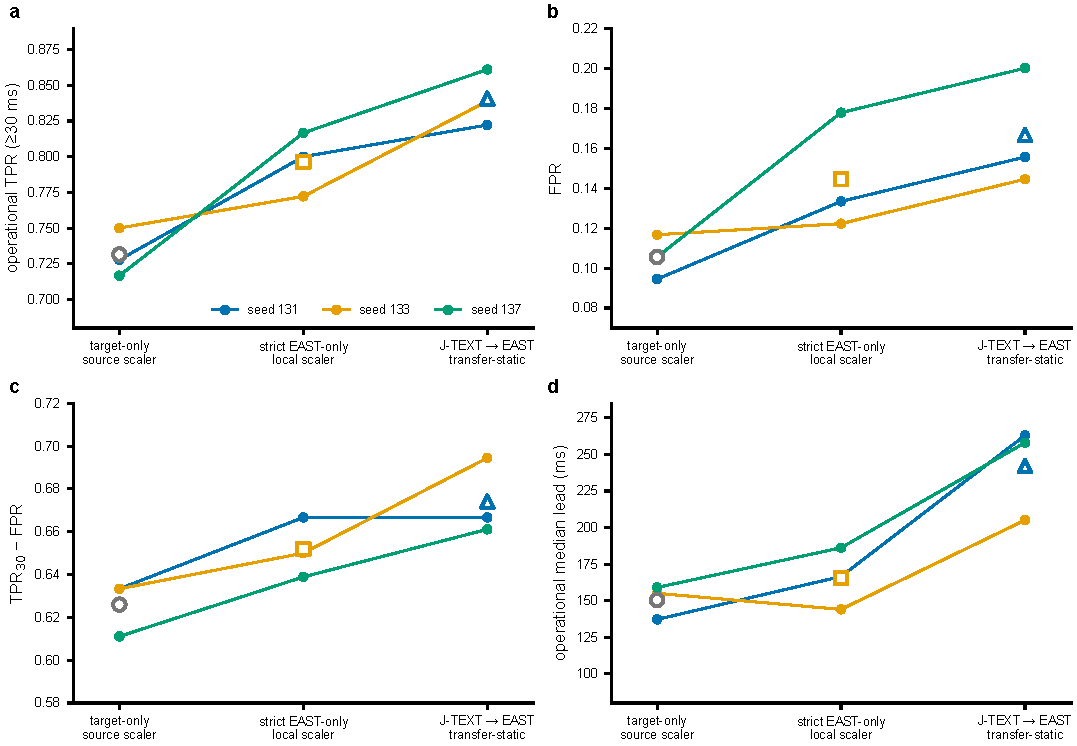
\includegraphics[width=\linewidth]{fig10_target_only_vs_transfer.pdf}
  \caption{严格 EAST-only、仅复用源缩放器的目标模型与 J-TEXT 至 EAST 静态迁移的三随机种子比较。}
  \label{fig:target-only-transfer}
\end{figure}
支持集只使用 110 炮 HDF5 真标签。全部 110 炮同时用于目标组件拟合和 support-derived 阈值（名义 support TPR=0.8）选择，没有独立 EAST validation；其中只有15个破裂结局，因此任何 target 泛化解释都必须降级为开发证据。有效路线不是全局无条件域对齐，而是：


\begin{ReportVerbatim}
J-TEXT rebuilt17 Transformer
→ EAST adapt_high 高层时间/风险适配
→ EAST DynamicHazardAdapter
→ EAST-private raw8 sidecar
→ 支持集阈值与双分支因果告警
\end{ReportVerbatim}

DynamicHazardAdapter 使用冻结 CLS、末 token、lag-8 增量及可用物理族摘要，参数量 3,893，风险残差限制在 \texttt{[-1,1]}\allowbreak{}。正残差需通过 support 正例分位数门。源 checkpoint 和冻结基座在运行前后做 SHA 比较。

三 seed 静态 balanced360：


{\scriptsize
\renewcommand{\arraystretch}{1.18}
\begin{xltabular}{\textwidth}{@{}>{\RaggedRight\arraybackslash}X>{\RaggedRight\arraybackslash}X>{\RaggedRight\arraybackslash}X>{\RaggedRight\arraybackslash}X>{\RaggedRight\arraybackslash}X>{\RaggedRight\arraybackslash}X@{}}
\toprule
\rowcolor{auditblue!10}
seed & TP30/\allowbreak{}FP/\allowbreak{}FN30/\allowbreak{}TN & operational TPR & FPR & operational median lead & >3s \\
\midrule
\endfirsthead
\toprule
\rowcolor{auditblue!10}
seed & TP30/\allowbreak{}FP/\allowbreak{}FN30/\allowbreak{}TN & operational TPR & FPR & operational median lead & >3s \\
\midrule
\endhead
131 & 148/\allowbreak{}28/\allowbreak{}32/\allowbreak{}152 & 0.8222 & 0.1556 & 263.0 ms & 22 \\
133 & 151/\allowbreak{}26/\allowbreak{}29/\allowbreak{}154 & 0.8389 & 0.1444 & 205.1 ms & 20 \\
137 & 155/\allowbreak{}36/\allowbreak{}25/\allowbreak{}144 & 0.8611 & 0.2000 & 258.0 ms & 21 \\
\bottomrule
\end{xltabular}
}

根据本项目预先确定的评价口径，提前量大于3,000 ms 的报警仍计入 TPR。报告同时单列此类报警数量，以避免将极早报警直接解释为已获得物理验证的破裂前兆。


\FloatBarrier
\section{EAST 因果在线适配}

\begin{figure}[htbp]
  \centering
  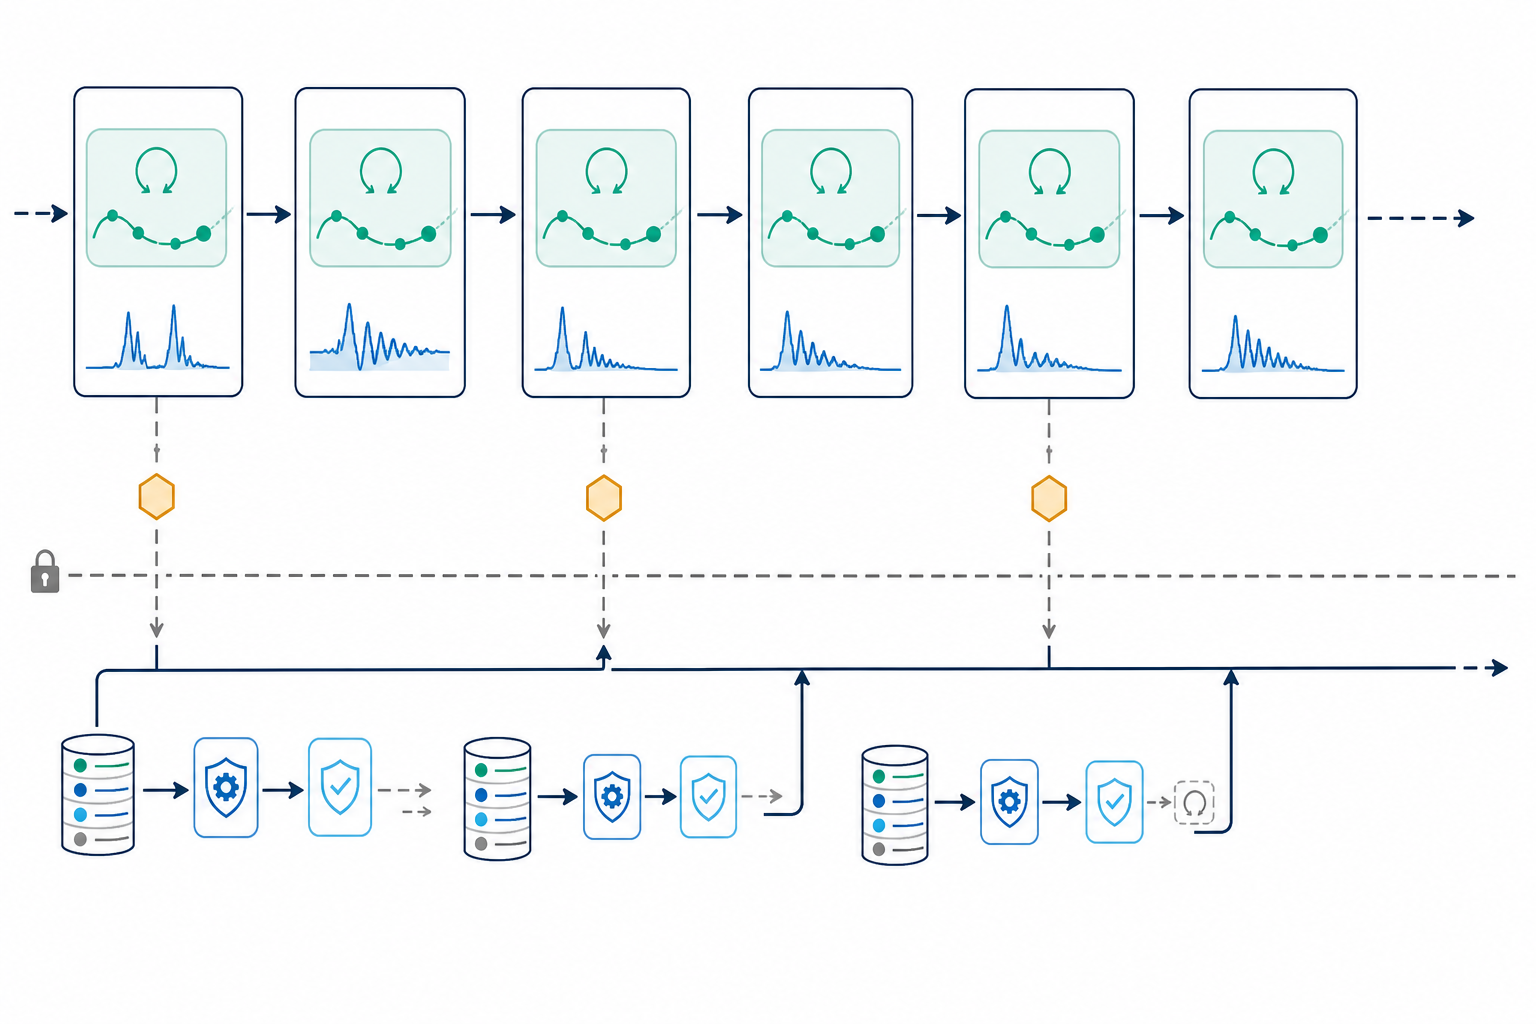
\includegraphics[width=0.80\linewidth]{concept_causal_online_v1.png}
  \caption{炮内临时适配、稀疏查询、信息边界、保护更新与回滚的概念示意。该图由生成式图像工具制作，仅表达方法结构，不包含测量数据、模型输出或实验数值。}
  \label{fig:concept-causal-online}
\end{figure}

\subsection{严格因果顺序}
每炮执行：


\begin{ReportVerbatim}
只看当前及过去窗口做无标签炮内更新
→ 输出并封存当前炮风险、告警、模型哈希和查询分
→ 不读标签决定是否查询
→ 仅被查询炮读取 HDF5 结局和 DownTime
→ 按 FP/FN/TARDY/TP/TN 形成炮后监督
→ guard + replay + accept/rollback
→ 更新只影响下一炮
\end{ReportVerbatim}

静态阶段先一次性跑完并关闭文件；在线阶段从完全相同的迁移父模型重置。这样“静态模型看过全 360 标签后再在线”的泄漏不存在。

A1 辅助入口也已改为严格 feature-only 流：训练只读取 support110；预测当前360炮时只读取信号与采样元数据，不打开 \texttt{IsDisrupt}\texttt{/\allowbreak{}}\allowbreak{}\texttt{DownTime}\allowbreak{}。惰性 oracle 仅在当前炮预测封存且查询决策为真后读取该炮结局；未查询炮直到整条流结束后的最终评估才读取。


\subsection{四类价值函数}
当前架构不再让一个标量同时控制所有动作。


\begin{enumerate}
\item \textbf{炮内无标签价值}：下一物理状态重建、教师分歧、物理冲突、raw8 innovation、availability、非冗余和告警接近度共同缩放 fast update；只用当前及过去窗口，下一炮前重置。
\item \textbf{查询价值}：执行分数由 uncertainty 与 physics contradiction 组成；过去分数的滚动分位数按 20 炮块冻结，rolling token bucket 控制长期平均查询率。配置中的 \texttt{query\_\allowbreak{}quota=6}\allowbreak{} 在 shadow/\allowbreak{}legacy 路径中是每 20 炮的 token 补充率，不是硬性逐块上限；实际单块可短时突发到 11 炮，但总查询数仍为 102/\allowbreak{}90/\allowbreak{}99。五专家复杂价值只做 shadow 审计，因为 v3a 让它直接接管查询后 operational TPR 下降。
\item \textbf{炮后梯度价值}：HDF5 揭示后比较封存预测与真实时序状态；FN/\allowbreak{}TARDY 优先选择 30--125 ms 内最接近跨过告警边界的窗口，而不是选择最难学习的最低风险点；固定两步更新，学习率由价值缩放。
\item \textbf{报警 episode 价值}：用 \texttt{delta60}\allowbreak{} 因果片段表示和过去已查询标签学习 FP 概率，只允许延迟或 veto，不允许创造或提前告警；独立物理支持可以 escape。
\end{enumerate}


\subsection{Q30 与主在线查询预算的关系}
项目记录中的“主动选择30炮”和“冻结30炮清单”分别对应 Q30 实验的在线选择阶段与后续受控消融阶段，二者在时间顺序和用途上并不冲突：


{\footnotesize
\renewcommand{\arraystretch}{1.18}
\begin{xltabular}{\textwidth}{@{}>{\RaggedRight\arraybackslash}X>{\RaggedRight\arraybackslash}X>{\RaggedRight\arraybackslash}X>{\RaggedRight\arraybackslash}X>{\RaggedRight\arraybackslash}X@{}}
\toprule
\rowcolor{auditblue!10}
对象 & 标签数 & 如何产生 & 后续如何使用 & 评估集合 \\
\midrule
\endfirsthead
\toprule
\rowcolor{auditblue!10}
对象 & 标签数 & 如何产生 & 后续如何使用 & 评估集合 \\
\midrule
\endhead
seed131 低预算 Q30 & 30 & 按 balanced360 时间顺序执行；每炮先预测并封存，再由只读当前/\allowbreak{}过去特征的查询价值与滚动预算即时决定是否查询 & 选择完成后冻结为同一 manifest，供 \texttt{inter}\texttt{\_}\allowbreak{}\texttt{only}\allowbreak{}、\texttt{intra}\texttt{+}\allowbreak{}\texttt{inter}\allowbreak{} 和30炮前置迁移复用 & 全360的时序消融；涉及前置训练时只评估未训练的330炮 \\
当前主在线 v3c & 102/\allowbreak{}90/\allowbreak{}99 & 三个 seed 各自在流中自适应查询；不是固定30炮 & 形成论文主在线结果及相应的炮后更新 & 各自完整 chronological balanced360 开发流 \\
同标签预算前置迁移 v2 & 102/\allowbreak{}90/\allowbreak{}99 & 不重新选炮；读取每个 seed 已封存的主在线查询清单 & 将查询标签一次性前置加入目标域训练，作为标签访问量对照 & 分别排除训练炮后的258/\allowbreak{}270/\allowbreak{}261炮 \\
因果随机查询对照 & 与主在线逐块标签数相同 & 标签不可见的块匹配随机日程，每 seed 三次重复 & 使用相同父模型、runner 和配置更新预算 & balanced360 开发流 \\
\bottomrule
\end{xltabular}
}

因此，Q30 既不是事先人工指定的固定 cohort，也不是观察完整360炮后离线选出的“全局最高价值30炮”。其严格定义是：每一炮到达后，系统仅依据当时可见信息、由历史分数形成的动态阈值、滚动 token 预算和探索规则，因果地决定是否支付标注成本；已经执行的早期查询不会因未来出现更高分样本而撤销。选择阶段结束后冻结 Q30 清单，仅用于保证各消融实验访问完全相同的标签集合。

当前包已保存 Q30 的30个炮号、流位置、\texttt{label\_\allowbreak{}oracle\_\allowbreak{}used=false}\allowbreak{} 和来源哈希；但 2026-08-21 tmpfs 重启后原始360行 \texttt{query}\texttt{\_}\allowbreak{}\texttt{decisions}\texttt{.}\allowbreak{}\texttt{jsonl}\allowbreak{} 未恢复，只保留其 SHA256。因此可以审计“冻结清单是什么”和“没有声明标签 oracle”，却不能仅凭现存包逐炮重算原始 cutoff、价值分数与 exploration/\allowbreak{}exploitation 路由。Q30 结论必须保留为 seed131 的开发性诊断，不能替代主在线三 seed 结果，也不能作为独立确认。


\subsection{多参数报警函数和状态机}

\begin{figure}[htbp]
  \centering
  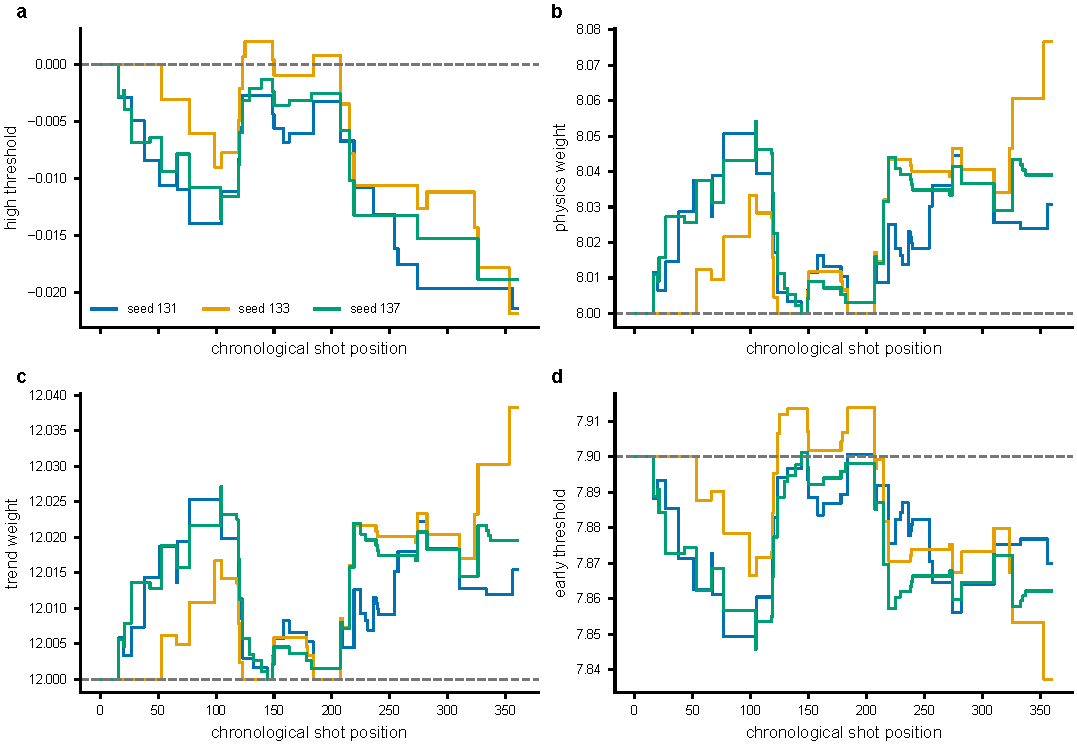
\includegraphics[width=\linewidth]{fig5_adaptive_alarm_state_machine.pdf}
  \caption{四个报警状态参数在 balanced360 顺序开发流中的真实演化轨迹。参数只在已查询炮揭示后更新，并受投影边界约束。}
  \label{fig:alarm-state}
\end{figure}
当前开发流中执行的报警器不是单一 max threshold；它尚未经过装置侧部署验收。每个因果时刻 (t) 使用两条路径：


\begin{ReportVerbatim}
high route:
  margin_t >= high_threshold

early route:
  margin_t
  + physics_weight * physics_support_t
  + trend_weight * max(MA5(margin)_t - MA100(margin)_t, 0)
  >= early_threshold
\end{ReportVerbatim}

四个连续参数受投影边界约束并允许在被查询炮揭示后更新；快慢窗口 \texttt{5}\texttt{/\allowbreak{}}\allowbreak{}\texttt{100}\allowbreak{} 固定，防止在线改变历史算子的语义。FP 使阈值更严格，FN/\allowbreak{}TARDY 使阈值更早并加强物理/\allowbreak{}趋势证据，TP/\allowbreak{}TN 则进入保护 guard。候选更新只要破坏任一已保护正确轨迹就回滚。episode gate 位于双路径之后，只能延迟或否决，不能创建或提前报警。

冻结日志证明参数确实在线变化，而不是只在配置中存在：


{\footnotesize
\renewcommand{\arraystretch}{1.18}
\begin{xltabular}{\textwidth}{@{}>{\RaggedRight\arraybackslash}X>{\RaggedRight\arraybackslash}X>{\RaggedRight\arraybackslash}X>{\RaggedRight\arraybackslash}X>{\RaggedRight\arraybackslash}X@{}}
\toprule
\rowcolor{auditblue!10}
seed & 查询/\allowbreak{}更新事件 & 实际改变参数 & 初始 \texttt{(h, wp, wt, e)}\allowbreak{} & 最终 \texttt{(h, wp, wt, e)}\allowbreak{} \\
\midrule
\endfirsthead
\toprule
\rowcolor{auditblue!10}
seed & 查询/\allowbreak{}更新事件 & 实际改变参数 & 初始 \texttt{(h, wp, wt, e)}\allowbreak{} & 最终 \texttt{(h, wp, wt, e)}\allowbreak{} \\
\midrule
\endhead
131 & 102 & 38 & \texttt{(0, 8, 12, 7.9)}\allowbreak{} & \texttt{(-0.02138, 8.03083, 12.01541, 7.86988)}\allowbreak{} \\
133 & 90 & 30 & \texttt{(0, 8, 12, 7.9)}\allowbreak{} & \texttt{(-0.02180, 8.07657, 12.03828, 7.83735)}\allowbreak{} \\
137 & 99 & 40 & \texttt{(0, 8, 12, 7.9)}\allowbreak{} & \texttt{(-0.01883, 8.03904, 12.01952, 7.86219)}\allowbreak{} \\
\bottomrule
\end{xltabular}
}

在当前炮预测时，系统不知道未来 DownTime；炮后揭示才把结果分成 TP、TN、FP、FN 或 TARDY。TARDY 表示“报警但 lead<30ms”，在正式评价中与 FN 一样是 operational error，并推动后续炮更早报警。


\subsection{动态误报保护}

\begin{figure}[htbp]
  \centering
  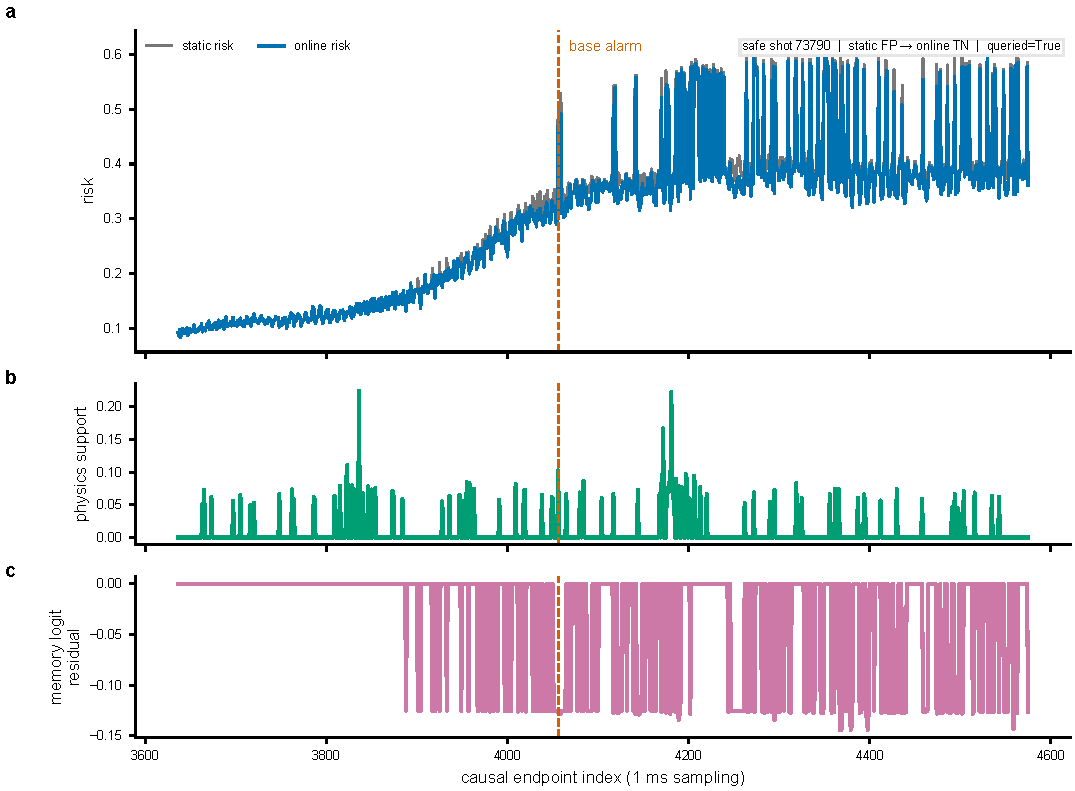
\includegraphics[width=\linewidth]{fig6_causal_false_alarm_rescue_shot73790.pdf}
  \caption{安全炮73790的开发性案例分析：风险、物理支持与因果 episode veto 的关系。单炮案例不构成总体泛化证据。}
  \label{fig:false-alarm-case}
\end{figure}
跨 seed 固定 \texttt{p(FP)>0.85}\allowbreak{} 曾失败。最终阈值只从过去已查询历史构造：


\begin{ReportVerbatim}
tau_FP = max(0.50, past disruptive-class FP-score q0.90 + 0.06)
\end{ReportVerbatim}

只有它低于 past safe-class q0.25 且历史样本、类别和置信度充分时才启用；否则 fail-open。\texttt{physics\_\allowbreak{}support >= 0.85}\allowbreak{} 可以放行。操作告警和反事实学习告警相互隔离，避免“本炮被救成 TN 后反过来改变同炮学习组”造成后续轨迹泄漏。


\subsection{在线结果}

{\scriptsize
\renewcommand{\arraystretch}{1.18}
\begin{xltabular}{\textwidth}{@{}>{\RaggedRight\arraybackslash}X>{\RaggedRight\arraybackslash}X>{\RaggedRight\arraybackslash}X>{\RaggedRight\arraybackslash}X>{\RaggedRight\arraybackslash}X>{\RaggedRight\arraybackslash}X>{\RaggedRight\arraybackslash}X@{}}
\toprule
\rowcolor{auditblue!10}
seed & TP30/\allowbreak{}FP/\allowbreak{}FN30/\allowbreak{}TN & operational TPR & FPR & operational median lead & 查询数 & >3s \\
\midrule
\endfirsthead
\toprule
\rowcolor{auditblue!10}
seed & TP30/\allowbreak{}FP/\allowbreak{}FN30/\allowbreak{}TN & operational TPR & FPR & operational median lead & 查询数 & >3s \\
\midrule
\endhead
131 & 152/\allowbreak{}24/\allowbreak{}28/\allowbreak{}156 & 0.8444 & 0.1333 & 228.5 ms & 102 & 23 \\
133 & 151/\allowbreak{}24/\allowbreak{}29/\allowbreak{}156 & 0.8389 & 0.1333 & 214.0 ms & 90 & 20 \\
137 & 155/\allowbreak{}34/\allowbreak{}25/\allowbreak{}146 & 0.8611 & 0.1889 & 246.0 ms & 99 & 22 \\
\bottomrule
\end{xltabular}
}

三个 seed 合计相对各自静态模型减少 8 个 seed-shot FP，并增加 4 个 lead\ensuremath{\geq}30ms 的 operational TP。在线改为 TN 的安全炮为：


\begin{itemize}
\item seed131：73790、74928、76861、80801；
\item seed133：71060、74562；
\item seed137：74939、75135。
\end{itemize}


\FloatBarrier
\section{主动查询有效性分析}

{\footnotesize
\renewcommand{\arraystretch}{1.18}
\begin{xltabular}{\textwidth}{@{}>{\RaggedRight\arraybackslash}X>{\RaggedRight\arraybackslash}X>{\RaggedRight\arraybackslash}X>{\RaggedRight\arraybackslash}X>{\RaggedRight\arraybackslash}X@{}}
\toprule
\rowcolor{auditblue!10}
seed & 查询率 & 全流 operational error & 查询炮 error & 富集倍数 \\
\midrule
\endfirsthead
\toprule
\rowcolor{auditblue!10}
seed & 查询率 & 全流 operational error & 查询炮 error & 富集倍数 \\
\midrule
\endhead
131 & 28.3\% & 14.4\% & 34.3\% & 2.38\ensuremath{\times} \\
133 & 25.0\% & 14.7\% & 32.2\% & 2.19\ensuremath{\times} \\
137 & 27.5\% & 16.4\% & 41.4\% & 2.53\ensuremath{\times} \\
\bottomrule
\end{xltabular}
}

根据流结束后统一揭示的标签，被查询炮中的 operational error 比例高于全流，表明查询策略对潜在错误炮具有事后富集。项目已补充 causal random-query 在线对照；由于查询分数和策略均曾在 balanced360 上开发，且仅有三个模型 seed，该结果只能支持开发流内的方向性比较，不能作为确认性显著性证据。


\subsection{同查询标签预算前置训练消融}

\begin{figure}[htbp]
  \centering
  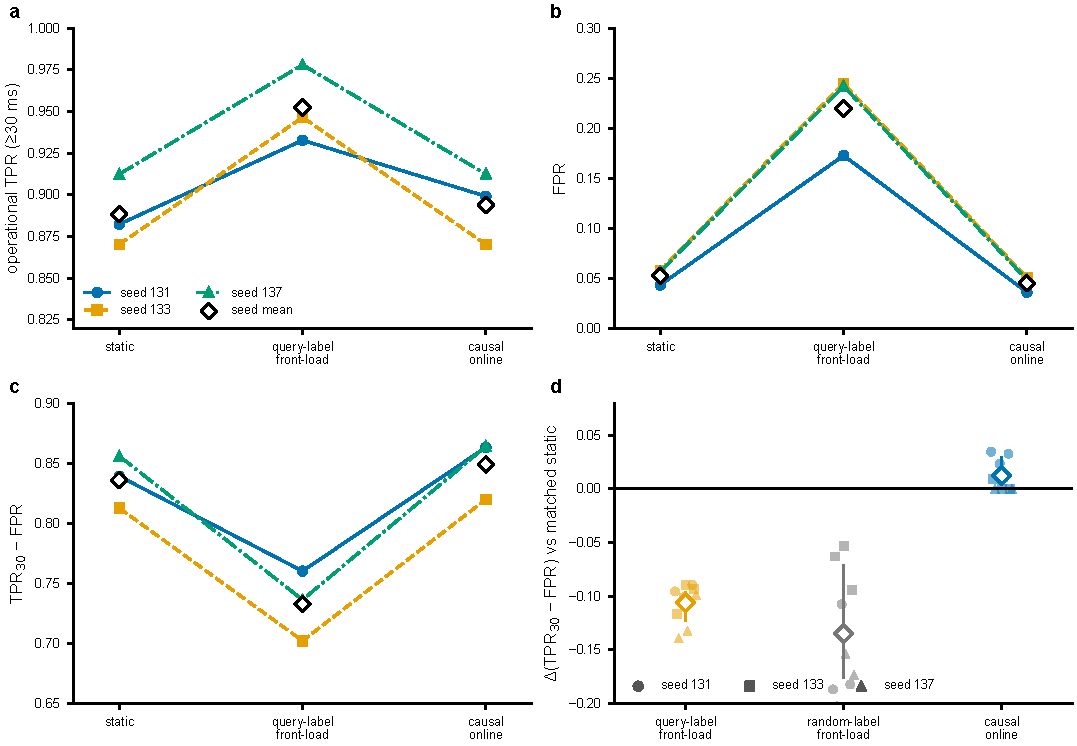
\includegraphics[width=\linewidth]{fig8_equal_label_budget_frontload_ablation.pdf}
  \caption{同标签访问量前置训练消融。评分严格排除被用于前置训练的查询炮；普通前置重训提高灵敏度的同时显著扩大误报。}
  \label{fig:frontload-ablation}
\end{figure}
为排除“在线主动只是因为多看了 EAST 标签”这一替代解释，针对每个 seed 读取其真实查询炮身份，把这些炮的 HDF5 标签在流开始前直接加入普通迁移重训。所有被加入训练的查询炮随后从该 seed 的评分集合剔除；静态模型、前置重训模型和因果在线模型只在完全相同的标签不相交补集上比较。

正式比较前先执行父模型复现门；support110-only 重训所得的各模块 SHA256、阈值和静态预测必须与历史最佳父模型完全一致。早期 v1 因后来采样器从“先抽炮、再在炮内抽窗口”漂移成“先抽类别、再抽炮”而未通过复现门，已标记 \texttt{INVALID}\texttt{\_}\allowbreak{}\texttt{PARENT}\texttt{\_}\allowbreak{}\texttt{FIDELITY}\allowbreak{}，不进入结论。


{\scriptsize
\renewcommand{\arraystretch}{1.18}
\begin{xltabular}{\textwidth}{@{}>{\RaggedRight\arraybackslash}X>{\RaggedRight\arraybackslash}X>{\RaggedRight\arraybackslash}X>{\RaggedRight\arraybackslash}X>{\RaggedRight\arraybackslash}X>{\RaggedRight\arraybackslash}X@{}}
\toprule
\rowcolor{auditblue!10}
seed & 查询 D/\allowbreak{}N & 评分 D/\allowbreak{}N & 静态 TPR30/\allowbreak{}FPR/\allowbreak{}J & 查询标签前置 TPR30/\allowbreak{}FPR/\allowbreak{}J & 在线 TPR30/\allowbreak{}FPR/\allowbreak{}J \\
\midrule
\endfirsthead
\toprule
\rowcolor{auditblue!10}
seed & 查询 D/\allowbreak{}N & 评分 D/\allowbreak{}N & 静态 TPR30/\allowbreak{}FPR/\allowbreak{}J & 查询标签前置 TPR30/\allowbreak{}FPR/\allowbreak{}J & 在线 TPR30/\allowbreak{}FPR/\allowbreak{}J \\
\midrule
\endhead
131 & 61/\allowbreak{}41 & 119/\allowbreak{}139 & 0.8824/\allowbreak{}0.0432/\allowbreak{}0.8392 & 0.9328/\allowbreak{}0.1727/\allowbreak{}0.7601 & 0.8992/\allowbreak{}0.0360/\allowbreak{}0.8632 \\
133 & 49/\allowbreak{}41 & 131/\allowbreak{}139 & 0.8702/\allowbreak{}0.0576/\allowbreak{}0.8127 & 0.9466/\allowbreak{}0.2446/\allowbreak{}0.7020 & 0.8702/\allowbreak{}0.0504/\allowbreak{}0.8199 \\
137 & 43/\allowbreak{}56 & 137/\allowbreak{}124 & 0.9124/\allowbreak{}0.0565/\allowbreak{}0.8560 & 0.9781/\allowbreak{}0.2419/\allowbreak{}0.7362 & 0.9124/\allowbreak{}0.0484/\allowbreak{}0.8640 \\
等 seed 均值 & --- & --- & 0.8883/\allowbreak{}0.0524/\allowbreak{}0.8359 & 0.9525/\allowbreak{}0.2197/\allowbreak{}0.7327 & 0.8939/\allowbreak{}0.0449/\allowbreak{}0.8490 \\
\bottomrule
\end{xltabular}
}

这里 \texttt{J = TPR@30ms \ensuremath{-} FPR}\allowbreak{}，只是显式的平衡操作点摘要。查询标签前置重训相对静态的变化为：


\begin{ReportVerbatim}
ΔTPR@30 = +0.0641
ΔFPR    = +0.1673
ΔJ      = -0.1032
\end{ReportVerbatim}

三个 seed 的方向完全一致：查询标签前置后召回、AUC 和提前量上升，但大量安全炮同时越过报警边界；在线模型相对该前置模型的 \texttt{\ensuremath{\Delta}J=+0.1163}\allowbreak{}。即使使用 support110 重新选择阈值，前置模型的 $J$ 仍降至 \texttt{0}\texttt{.}\allowbreak{}\texttt{7252}\allowbreak{}，说明该退化不能通过目标阈值重标定消除。

另做每 20 炮查询数严格匹配、完全不读取标签的 random front-load，每 seed 三个重复，并先在 seed 内平均。common-mask 的静态、selected front-load、random front-load、在线 J 分别为 \texttt{0}\texttt{.}\allowbreak{}\texttt{8387}\texttt{/\allowbreak{}}\allowbreak{}\texttt{0}\texttt{.}\allowbreak{}\texttt{7322}\texttt{/\allowbreak{}}\allowbreak{}\texttt{0}\texttt{.}\allowbreak{}\texttt{7033}\texttt{/\allowbreak{}}\allowbreak{}\texttt{0}\texttt{.}\allowbreak{}\texttt{8510}\allowbreak{}。因此可以排除“标签数量本身足以解释在线操作点”；结果更符合延迟的错误类型更新、受限步长、support replay、rollback 与报警状态保护共同作用。

该前置消融仍不构成最终因果证明：balanced360 参与了方法开发；前置重训只实现 label-access matched，历史在线日志未完整保存精确窗口索引、optimizer/\allowbreak{}RNG 状态和 FLOPs，因而无法执行 exact equal-gradient replay；同时仅有三个模型 seed，三次同向结果对应的单侧精确 sign-test 概率为0.125，不满足确认性显著性要求。


\subsection{因果随机查询在线对照}

\begin{figure}[htbp]
  \centering
  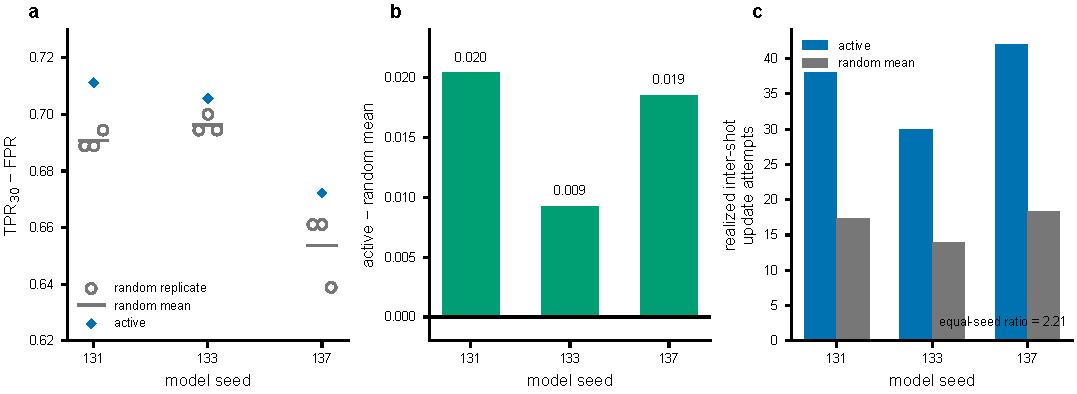
\includegraphics[width=\linewidth]{fig9_active_vs_causal_random_query.pdf}
  \caption{主动查询与按20炮块匹配标签数的因果随机查询对照。实际更新尝试数不相等，因此该图描述完整耦合机制，而非严格等 FLOPs 的选择器效应。}
  \label{fig:active-random}
\end{figure}
另从每个真实主动查询账本构造三条不读取标签的随机查询轨：每20炮查询数、总查询数、父模型、静态预测、runner和配置的optimizer-step上限均与主动臂一致。随机身份在预测前固定，每炮仍严格执行 \texttt{predict \ensuremath{\rightarrow} seal \ensuremath{\rightarrow} query \ensuremath{\rightarrow} reveal \ensuremath{\rightarrow} update}\allowbreak{}。


{\footnotesize
\renewcommand{\arraystretch}{1.18}
\begin{xltabular}{\textwidth}{@{}>{\RaggedRight\arraybackslash}X>{\RaggedRight\arraybackslash}X>{\RaggedRight\arraybackslash}X>{\RaggedRight\arraybackslash}X@{}}
\toprule
\rowcolor{auditblue!10}
seed & 主动 J & 随机 J（3重复均值） & 主动\ensuremath{-}随机 \\
\midrule
\endfirsthead
\toprule
\rowcolor{auditblue!10}
seed & 主动 J & 随机 J（3重复均值） & 主动\ensuremath{-}随机 \\
\midrule
\endhead
131 & 0.7111 & 0.6907 & +0.0204 \\
133 & 0.7056 & 0.6963 & +0.0093 \\
137 & 0.6722 & 0.6537 & +0.0185 \\
等 seed 均值 & 0.6963 & 0.6802 & +0.0160 \\
\bottomrule
\end{xltabular}
}

三个 seed 方向一致，但不能写成“同计算量主动选择已被显著证明”：主动臂平均发生36.67次共享炮间更新尝试，随机臂为16.56次，比值2.21。错误触发更多更新既是主动机制的一部分，也是实现计算量的中介变量；精确三符号单侧概率仍为0.125。该对照关闭了“根本没有causal random在线基线”的缺口，但没有关闭严格等FLOPs隔离和未来流确认缺口。


\subsection{固定窗口、batch形状与optimizer-attempt的查询名单对照}

\begin{figure}[htbp]
  \centering
  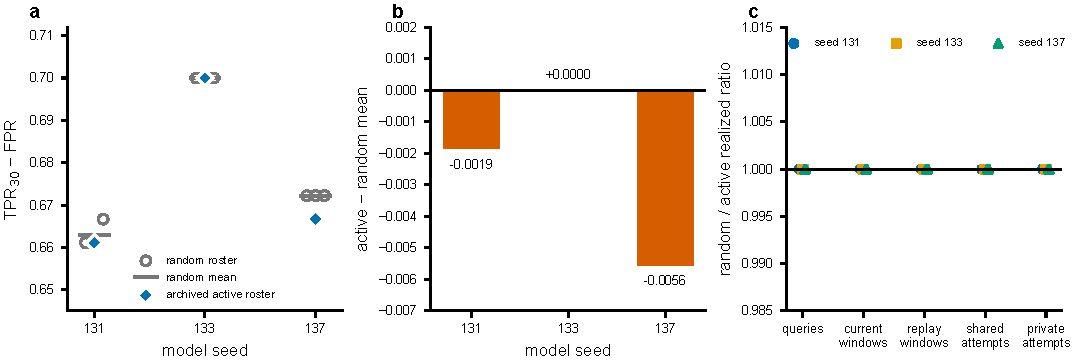
\includegraphics[width=\linewidth]{fig11_equal_compute_selector_screen.pdf}
  \caption{固定窗口、批形状和 optimizer-attempt 的查询名单筛查。归档主动名单在该固定同化算子下未显示稳定优于随机名单。}
  \label{fig:equal-compute}
\end{figure}
为隔离上一节的实现计算量中介，另建立一个\textbf{不同于主在线机制}的固定同化算子。它从同一迁移父模型和同一静态360账本出发，只比较“归档主动查询名单”与“标签不可见、每20炮查询数匹配的随机名单”。炮内更新、报警参数学习、episode gate、query-value learner、error memory 和 typed memory 全部冻结。每个被查询炮无论事后属于 TP/\allowbreak{}TN/\allowbreak{}FP/\allowbreak{}FN/\allowbreak{}TARDY，均强制执行：


\begin{ReportVerbatim}
16个当前炮监督窗口 + 16个固定support110回放窗口
→ shared adapter恰好2个optimizer attempts
→ private adapter恰好2个optimizer attempts
→ 当前炮预测已封存；参数只能影响下一炮及以后
\end{ReportVerbatim}

逐炮回执记录窗口索引、batch shape、可训练参数scope hash、尝试/\allowbreak{}提交/\allowbreak{}回滚步数和首次可影响的下一炮。三个 seed 的实际预算分别为：


{\scriptsize
\renewcommand{\arraystretch}{1.18}
\begin{xltabular}{\textwidth}{@{}>{\RaggedRight\arraybackslash}X>{\RaggedRight\arraybackslash}X>{\RaggedRight\arraybackslash}X>{\RaggedRight\arraybackslash}X>{\RaggedRight\arraybackslash}X>{\RaggedRight\arraybackslash}X>{\RaggedRight\arraybackslash}X@{}}
\toprule
\rowcolor{auditblue!10}
seed & 查询数 & 当前/\allowbreak{}回放窗口总数 & shared/\allowbreak{}private attempts & 主动 J & 随机 J（3重复均值） & 主动\ensuremath{-}随机 \\
\midrule
\endfirsthead
\toprule
\rowcolor{auditblue!10}
seed & 查询数 & 当前/\allowbreak{}回放窗口总数 & shared/\allowbreak{}private attempts & 主动 J & 随机 J（3重复均值） & 主动\ensuremath{-}随机 \\
\midrule
\endhead
131 & 102 & 1632 /\allowbreak{} 1632 & 204 /\allowbreak{} 204 & 0.6611 & 0.6630 & -0.00185 \\
133 & 90 & 1440 /\allowbreak{} 1440 & 180 /\allowbreak{} 180 & 0.7000 & 0.7000 & 0 \\
137 & 99 & 1584 /\allowbreak{} 1584 & 198 /\allowbreak{} 198 & 0.6667 & 0.6722 & -0.00556 \\
\bottomrule
\end{xltabular}
}

事后开发阶段明确写入报告的初筛规则是三个 seed 上主动名单都优于随机均值；它没有独立时间戳预注册凭据。结果为 \texttt{0}\texttt{/\allowbreak{}}\allowbreak{}\texttt{3}\allowbreak{} seed 通过，等 seed 平均差为 \texttt{-}\allowbreak{}\texttt{0}\texttt{.}\allowbreak{}\texttt{00247}\allowbreak{}。因此必须撤回“查询身份本身已经被证明优于随机”的论点。可支持的较窄结论是：在这个新固定同化算子下，没有观察到归档主动名单相对三条随机名单的稳定优势；该实验不估计原自适应选择策略的政策效应。主在线结果仍只能作为查询身份、错误触发更新强度、同错回放、rollback、报警状态保护和 episode veto 的\textbf{耦合处理效应}汇报。

这个负结果不等于证明主动与随机等价，也不等于所有可能同化算子下查询价值无效。原因是只有三个随机日程、balanced360 已参与开发，而且归档主动身份是一个固定 roster treatment，并非在新流上重新执行自适应策略。它只使“这个固定算子下的归档名单优越性”论点失败，不能否定查询身份在原耦合机制中的贡献，也不能给出普遍零效应或确认性统计结论。完整证据见 \texttt{evidence}\texttt{/\allowbreak{}}\allowbreak{}\texttt{equal}\texttt{\_}\allowbreak{}\texttt{compute}\texttt{\_}\allowbreak{}\texttt{selector}\texttt{\_}\allowbreak{}\texttt{control}\texttt{\_}\allowbreak{}\texttt{v1}\texttt{/\allowbreak{}}\allowbreak{}\texttt{report}\texttt{.}\allowbreak{}\texttt{json}\allowbreak{}。


\FloatBarrier
\section{负对照与失败实验记录}

\begin{figure}[htbp]
  \centering
  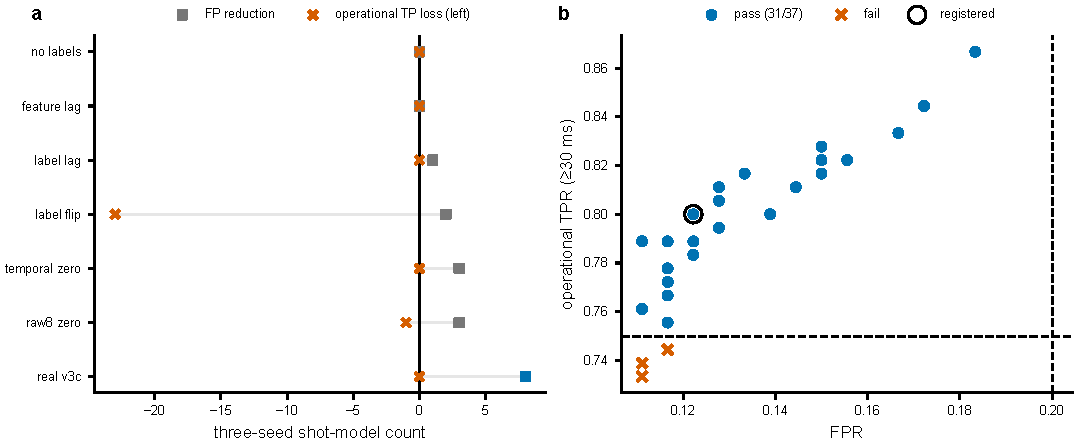
\includegraphics[width=\linewidth]{fig7_negative_controls_and_alarm_robustness.pdf}
  \caption{负对照和前置报警器参数鲁棒性。负对照用于限制机制解释；鲁棒性结果不替代最终在线链路的独立验证。}
  \label{fig:negative-controls}
\end{figure}

{\footnotesize
\renewcommand{\arraystretch}{1.18}
\begin{xltabular}{\textwidth}{@{}>{\RaggedRight\arraybackslash}X>{\RaggedRight\arraybackslash}X>{\RaggedRight\arraybackslash}X>{\RaggedRight\arraybackslash}X@{}}
\toprule
\rowcolor{auditblue!10}
对照 & 三 seed 总 FP 减少 & operational TP 损失 & 裁决 \\
\midrule
\endfirsthead
\toprule
\rowcolor{auditblue!10}
对照 & 三 seed 总 FP 减少 & operational TP 损失 & 裁决 \\
\midrule
\endhead
不揭示标签 & 0 & 0 & 无法形成保护边界 \\
特征错位一炮 & 0 & 0 & 表象相似不足以替代当前因果片段 \\
标签错位一炮 & 1 & 0 & 真实增益基本消失 \\
标签翻转 & 2 & 23 & 错标签会明显伤害合格报警 \\
时间演化特征置零 & 3 & 0 & 只保留部分增益 \\
名为 \texttt{raw8}\texttt{\_}\allowbreak{}\texttt{zero}\allowbreak{} 的归档episode/\allowbreak{}保护校准screen & 3 & 1 & 只说明该screen保留部分收益；未封存模型级sidecar干预和完整轨迹重跑，不能解释为八个私有通道的独立消融 \\
真实 v3c & 8 & 0 & 最大净收益且不损失合格报警 \\
\bottomrule
\end{xltabular}
}

这组对照支持“正确标签 \ensuremath{\times} 炮内时间演化 \ensuremath{\times} EAST 私有特征”共同作用，但不能证明网络学到了所有破裂因果机制。

开发阶段已停止继续投入的路线包括：raw23 无条件全局对齐；反复调节普通 DANN/\allowbreak{}MMD/\allowbreak{}CORAL 权重；对高维炮后 residual 直接提高学习率；由复杂价值函数未经隔离地接管查询；跨 seed 共用固定 FP 概率门；反馈未隔离的 veto；40\% 查询预算；以及将 PADFIX 父模型直接接入既有在线策略。停止依据均来自已归档的负迁移、操作灵敏度下降或无法隔离因果贡献等证据。


\FloatBarrier
\section{时间漂移与有效性风险}

\begin{figure}[htbp]
  \centering
  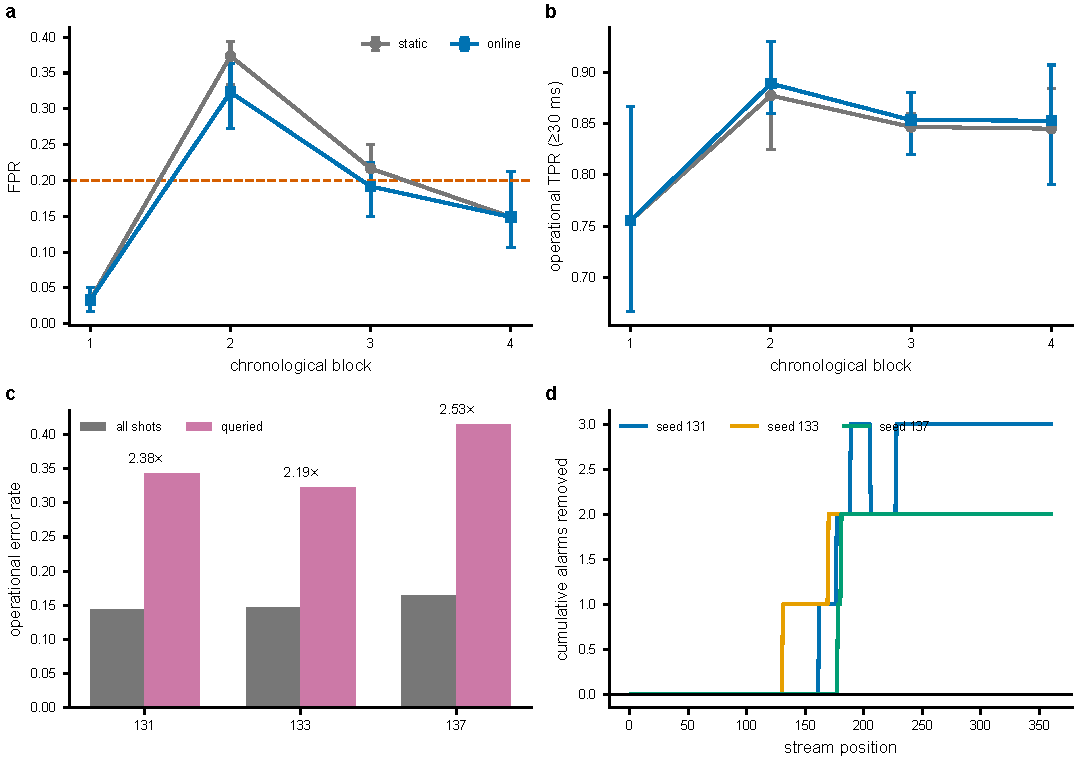
\includegraphics[width=\linewidth]{fig4_chronological_blocks_and_active_query_value.pdf}
  \caption{连续时间块异质性、查询错误富集和静态至在线累计报警变化。时间块结果揭示整体均值可能掩盖 campaign 漂移。}
  \label{fig:chronological-risk}
\end{figure}
把 balanced360 分成连续四个 90 炮块后，第二块 FPR 很高：


{\small
\renewcommand{\arraystretch}{1.18}
\begin{xltabular}{\textwidth}{@{}>{\RaggedRight\arraybackslash}X>{\RaggedRight\arraybackslash}X>{\RaggedRight\arraybackslash}X@{}}
\toprule
\rowcolor{auditblue!10}
seed & 在线 worst TPR@30 & 在线 worst FPR \\
\midrule
\endfirsthead
\toprule
\rowcolor{auditblue!10}
seed & 在线 worst TPR@30 & 在线 worst FPR \\
\midrule
\endhead
131 & 0.6667 & 0.2727 \\
133 & 0.7907 & 0.3333 \\
137 & 0.7333 & 0.3636 \\
\bottomrule
\end{xltabular}
}

safe score 与炮号的 Spearman 相关为 \texttt{0}\texttt{.}\allowbreak{}\texttt{220}\texttt{/\allowbreak{}}\allowbreak{}\texttt{0}\texttt{.}\allowbreak{}\texttt{091}\texttt{/\allowbreak{}}\allowbreak{}\texttt{0}\texttt{.}\allowbreak{}\texttt{311}\allowbreak{}，seed137 的 campaign/\allowbreak{}shot-state 风险明显。因此，整体均值不能替代分时间块稳定性审查，当前结果尚不足以支持跨 campaign 稳定性结论。

另一项主要有效性风险是源域 context shortcut。原 checkpoint 在同一 endpoint、仅删除更早历史的32/\allowbreak{}64/\allowbreak{}96/\allowbreak{}128点视图上表现如下：

| seed | padding probe AUC | mean |\ensuremath{\Delta}risk| | alarm flip | |---:|---:|---:|---:| | 131 | 0.955 | 0.061 | 5.70\% | | 133 | 0.929 | 0.064 | 8.55\% | | 137 | 0.937 | 0.071 | 7.02\% |

均未通过 \texttt{AUC\ensuremath{\leq}0.65、|\ensuremath{\Delta}risk|\ensuremath{\leq}0.05、flip\ensuremath{\leq}5\%}\allowbreak{}。


\FloatBarrier
\section{PADFIX 上下文捷径修复及负迁移}

\begin{figure}[htbp]
  \centering
  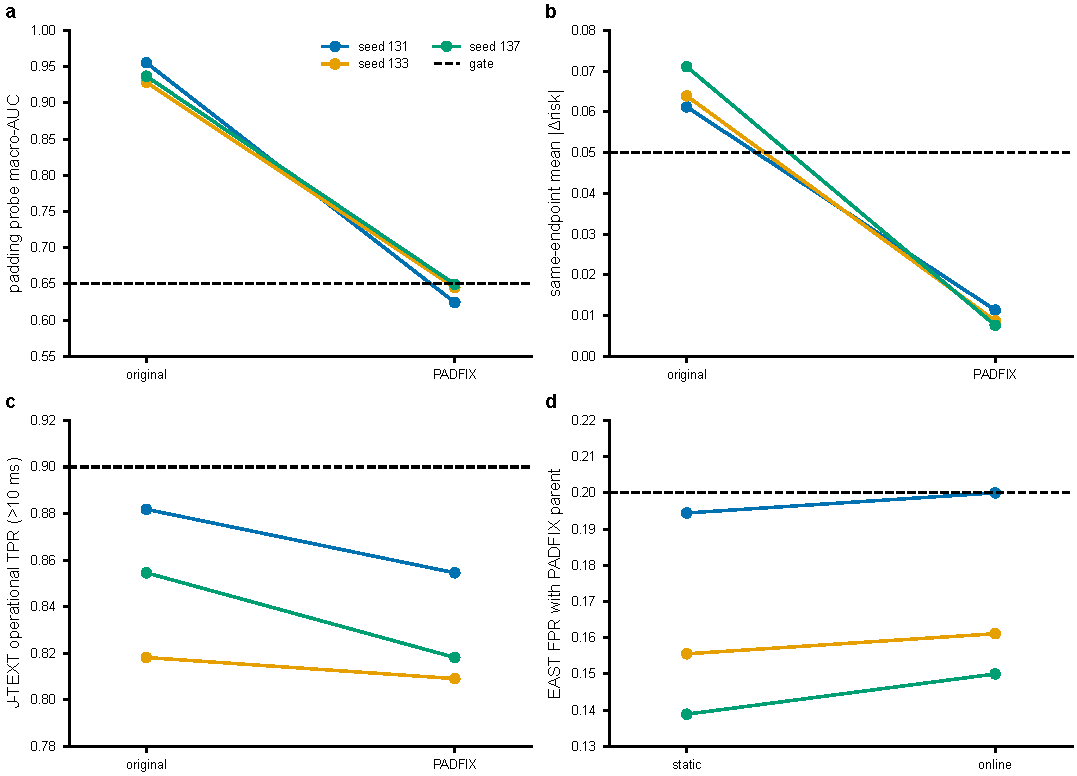
\includegraphics[width=\linewidth]{fig3_source_shortcut_and_padfix_tradeoff.pdf}
  \caption{源域上下文长度捷径与 PADFIX 权衡。PADFIX 降低 padding 可探测性，但直接沿用旧目标策略时发生负迁移。}
  \label{fig:padfix-tradeoff}
\end{figure}
PADFIX 为同一 endpoint 构造 \texttt{\{32,64,96,128\}}\allowbreak{} 合法短上下文，只删过去、不看未来，并加入风险一致性、表示一致性及按结局条件化的 padding 桶对抗项。三个 seed 的 VAL160 audit 全部过门：

| seed | probe AUC | mean |\ensuremath{\Delta}risk| | flip | |---:|---:|---:|---:| | 131 | 0.624 | 0.011 | 1.54\% | | 133 | 0.645 | 0.009 | 2.63\% | | 137 | 0.649 | 0.008 | 2.19\% |

但锁定后 TEST220 的平均 operational TPR@>10ms 变为 \texttt{0}\texttt{.}\allowbreak{}\texttt{8273}\allowbreak{}，FPR \texttt{0}\texttt{.}\allowbreak{}\texttt{1515}\allowbreak{}，AUC \texttt{0}\texttt{.}\allowbreak{}\texttt{9325}\allowbreak{}。把旧 target/\allowbreak{}online policy 原样接上时：


{\small
\renewcommand{\arraystretch}{1.18}
\begin{xltabular}{\textwidth}{@{}>{\RaggedRight\arraybackslash}X>{\RaggedRight\arraybackslash}X>{\RaggedRight\arraybackslash}X@{}}
\toprule
\rowcolor{auditblue!10}
阶段 & operational TPR@30 & FPR \\
\midrule
\endfirsthead
\toprule
\rowcolor{auditblue!10}
阶段 & operational TPR@30 & FPR \\
\midrule
\endhead
PADFIX \ensuremath{\rightarrow} EAST static & 0.8537 & 0.1630 \\
PADFIX \ensuremath{\rightarrow} EAST online & 0.8537 & 0.1704 \\
\bottomrule
\end{xltabular}
}

三个 seed 的在线 FPR 均上升。该结果不表示 PADFIX 对上下文捷径无效；它表明既有在线策略已适配原源模型的风险几何，不能在不重新验证的情况下迁移至新父模型。为控制 balanced360 上的进一步选择偏差，本轮终止参数重调。后续应在新增目标验证资源上独立选择与 PADFIX 匹配的目标策略，并在冻结后对新的未来流执行一次性确认。


\FloatBarrier
\section{报警参数鲁棒性}
前一版双阈值报警对 high threshold、physics weight、trend weight、early threshold、快慢均值窗做 37 个局部/\allowbreak{}联合扰动，31 个满足：


\begin{ReportVerbatim}
operational TPR@30 >= 0.75
FPR <= 0.20
\end{ReportVerbatim}

注册点为 operational TPR@30 \texttt{0}\texttt{.}\allowbreak{}\texttt{8000}\allowbreak{}、FPR \texttt{0}\texttt{.}\allowbreak{}\texttt{1222}\allowbreak{}、median lead \texttt{139 ms}\allowbreak{}。但 bootstrap 的 TPR@30 区间为 \texttt{[0.7389,0.8556]}\allowbreak{}，不足以支持“TPR 高置信度超过0.8”的表述。该试验只评价前置 alarm stage 的局部鲁棒性，不代表最终 v3c 全链路的鲁棒性。


\FloatBarrier
\section{图表与机器证据目录}
全部定量图由机器证据生成，使用色盲友好配色、183 mm 双栏宽、PDF/\allowbreak{}SVG 矢量和 600 dpi PNG；未使用生成式图片制造曲线或数据点。


\begin{enumerate}
\item \texttt{fig0}\texttt{\_}\allowbreak{}\texttt{end}\texttt{\_}\allowbreak{}\texttt{to}\texttt{\_}\allowbreak{}\texttt{end}\texttt{\_}\allowbreak{}\texttt{model}\texttt{\_}\allowbreak{}\texttt{architecture}\allowbreak{}：源域监督、共享迁移、EAST-private 支路与在线更新边界的总架构；
\item \texttt{fig1}\texttt{\_}\allowbreak{}\texttt{protocol}\texttt{\_}\allowbreak{}\texttt{and}\texttt{\_}\allowbreak{}\texttt{causal}\texttt{\_}\allowbreak{}\texttt{contract}\allowbreak{}：数据角色、迁移链路和在线因果顺序；
\item \texttt{fig2}\texttt{\_}\allowbreak{}\texttt{same}\texttt{\_}\allowbreak{}\texttt{lineage}\texttt{\_}\allowbreak{}\texttt{metrics}\texttt{\_}\allowbreak{}\texttt{and}\texttt{\_}\allowbreak{}\texttt{block}\texttt{\_}\allowbreak{}\texttt{resampling}\allowbreak{}：J-TEXT 源域指标与 EAST 静态\ensuremath{\rightarrow}在线配对变化分开呈现，禁止跨装置折线暗示，并给出 moving-block 描述区间；
\item \texttt{fig3}\texttt{\_}\allowbreak{}\texttt{source}\texttt{\_}\allowbreak{}\texttt{shortcut}\texttt{\_}\allowbreak{}\texttt{and}\texttt{\_}\allowbreak{}\texttt{padfix}\texttt{\_}\allowbreak{}\texttt{tradeoff}\allowbreak{}：padding shortcut 与 PADFIX 代价；
\item \texttt{fig4}\texttt{\_}\allowbreak{}\texttt{chronological}\texttt{\_}\allowbreak{}\texttt{blocks}\texttt{\_}\allowbreak{}\texttt{and}\texttt{\_}\allowbreak{}\texttt{active}\texttt{\_}\allowbreak{}\texttt{query}\texttt{\_}\allowbreak{}\texttt{value}\allowbreak{}：时间块漂移、错误富集和累计报警变化；
\item \texttt{fig5}\texttt{\_}\allowbreak{}\texttt{adaptive}\texttt{\_}\allowbreak{}\texttt{alarm}\texttt{\_}\allowbreak{}\texttt{state}\texttt{\_}\allowbreak{}\texttt{machine}\allowbreak{}：四个报警参数沿360炮顺序流的真实变化轨迹；
\item \texttt{fig6}\texttt{\_}\allowbreak{}\texttt{causal}\texttt{\_}\allowbreak{}\texttt{false}\texttt{\_}\allowbreak{}\texttt{alarm}\texttt{\_}\allowbreak{}\texttt{rescue}\texttt{\_}\allowbreak{}\texttt{shot73790}\allowbreak{}：安全炮 73790 的风险、物理支持和 episode veto；
\item \texttt{fig7}\texttt{\_}\allowbreak{}\texttt{negative}\texttt{\_}\allowbreak{}\texttt{controls}\texttt{\_}\allowbreak{}\texttt{and}\texttt{\_}\allowbreak{}\texttt{alarm}\texttt{\_}\allowbreak{}\texttt{robustness}\allowbreak{}：负对照与前置报警鲁棒性；
\item \texttt{fig8}\texttt{\_}\allowbreak{}\texttt{equal}\texttt{\_}\allowbreak{}\texttt{label}\texttt{\_}\allowbreak{}\texttt{budget}\texttt{\_}\allowbreak{}\texttt{frontload}\texttt{\_}\allowbreak{}\texttt{ablation}\allowbreak{}：同查询标签预算前置重训、随机前置与因果在线的配对消融；
\item \texttt{fig9}\texttt{\_}\allowbreak{}\texttt{active}\texttt{\_}\allowbreak{}\texttt{vs}\texttt{\_}\allowbreak{}\texttt{causal}\texttt{\_}\allowbreak{}\texttt{random}\texttt{\_}\allowbreak{}\texttt{query}\allowbreak{}：完整主动机制与因果块匹配随机查询的效用差异及实际更新尝试数；
\item \texttt{fig10}\texttt{\_}\allowbreak{}\texttt{target}\texttt{\_}\allowbreak{}\texttt{only}\texttt{\_}\allowbreak{}\texttt{vs}\texttt{\_}\allowbreak{}\texttt{transfer}\allowbreak{}：EAST-only、source-scaler target-only 和跨装置静态迁移的三 seed 比较；
\item \texttt{fig11}\texttt{\_}\allowbreak{}\texttt{equal}\texttt{\_}\allowbreak{}\texttt{compute}\texttt{\_}\allowbreak{}\texttt{selector}\texttt{\_}\allowbreak{}\texttt{screen}\allowbreak{}：固定16+16窗口、2+2 optimizer attempts（guard提交数可不同）算子下的查询名单负结果。
\end{enumerate}

\texttt{figure}\texttt{\_}\allowbreak{}\texttt{manifest}\texttt{.}\allowbreak{}\texttt{json}\allowbreak{} 保存所有输入和输出 SHA256。图 4 所需 NPZ 已复制进本论文包，不再依赖 \texttt{/\allowbreak{}}\allowbreak{}\texttt{home}\allowbreak{} 的个人工作目录。


\FloatBarrier
\section{结论适用范围}

\subsection{当前证据支持的表述}

\begin{itemize}
\item 在当前开发链及历史失败对照中，17 维语义共享 + 8 维 EAST 私有分支比继续强行无条件对齐 raw23 更可行；
\item 固定110炮能把 J-TEXT 表示重组为具有较高 EAST balanced360 TPR 的目标模型；
\item 在线执行在因果信息边界内完成，标签只影响后续炮；
\item 主动查询对 operational error 有约 2.2--2.5 倍内部富集；
\item 同查询标签直接前置重训会提高召回却显著扩大误报，不能复现在线的平衡操作点；
\item 最终 episode gate 在三个 seed 上同方向降低误报，且负对照不能保留完整增益；
\item 源模型 padding shortcut、PADFIX 负迁移和 campaign block 漂移是明确、可复现的失败发现。
\end{itemize}


\subsection{当前证据尚不支持的表述}

\begin{itemize}
\item “模型学到了所有破裂机理”；
\item “balanced360 是完全未见独立测试集”；
\item “已经部署通过”；
\item “三个 seed 等于1080个独立样本”；
\item “bootstrap 已证明未来 campaign 泛化”；
\item “PADFIX 已兼容当前 EAST 在线策略”；
\item “>3秒报警必然是有效物理前兆”。
\item “J-TEXT TEST220 是严格时序或真实患病率下的独立测试”；
\item “support110 提供了独立目标验证”；
\item “主动查询已在严格等FLOPs、独立未来流上显著优于随机查询”（当前只完成开发流内同标签数、同配置预算的 causal random-query 对照）。
\end{itemize}


\FloatBarrier
\section{前瞻确认实施方案}
在新 EAST 顺序流到来前，冻结：


\begin{itemize}
\item git SHA、环境、三 seed 源 checkpoint；
\item support110 roster/\allowbreak{}scaler/\allowbreak{}target parents；
\item alarm 公式、阈值、参数投影范围；
\item query 策略、预算、更新步数和 FLOPs；
\item v3c 配置与全部负对照；
\item PADFIX 是否作为独立候选及其目标策略选择规则。
\end{itemize}

新流逐炮只做一次：静态分支先完整封存；在线分支从相同父模型重置；每炮 predict/\allowbreak{}seal/\allowbreak{}query/\allowbreak{}reveal/\allowbreak{}update；所有炮必须报告，不能在失败后换阈值或删炮。只有三个 seed 在整体和最差时间块均通过，在线不退化，且随机/\allowbreak{}no-label/\allowbreak{}time-shift 等对照不能复现增益，才能把状态升级为独立确认。


\FloatBarrier
\section{证据成熟度与成果使用建议}
当前材料已达到“可审计研究开发稿”的完整度：标签、评价口径、因果顺序、逐炮账本、哈希、负结果和图表均可复查。该材料可用于项目阶段汇报、技术评审和后续论文方案论证；但其证据等级\textbf{尚不足以支撑确认性期刊主张或装置部署验收}。以下四项限制不能通过文字修订消除：


\begin{enumerate}
\item J-TEXT 主划分不是严格时序，VAL/\allowbreak{}TEST 是 count-aligned 平衡比较集；
\item EAST support110 同时用于拟合和阈值选择，缺少目标验证；
\item balanced360 用于972候选筛选，且没有完全未见未来流；
\item 严格等窗口/\allowbreak{}等optimizer-attempt查询名单对照已补齐，但主动名单未显示稳定优势；完整在线机制仍没有在独立未来流上做等计算确认，同时缺少可公开或受控访问的数据/\allowbreak{}代码 DOI。
\end{enumerate}

作者姓名、CRediT、经费、利益冲突和数据访问责任人也必须在投稿前补齐，不能由自动化工具推断。机器可读/\allowbreak{}逐项裁决见 \texttt{NATURE}\texttt{\_}\allowbreak{}\texttt{PORTFOLIO}\texttt{\_}\allowbreak{}\texttt{READINESS}\texttt{.}\allowbreak{}\texttt{md}\allowbreak{}。


\FloatBarrier
\section{交付物与复现入口}

\begin{itemize}
\item 英文主文：\texttt{manuscript}\texttt{/\allowbreak{}}\allowbreak{}\texttt{main}\texttt{.}\allowbreak{}\texttt{tex}\allowbreak{} 与编译后的 \texttt{manuscript}\texttt{/\allowbreak{}}\allowbreak{}\texttt{main}\texttt{.}\allowbreak{}\texttt{pdf}\allowbreak{}；
\item 英文补充材料：\texttt{manuscript}\texttt{/\allowbreak{}}\allowbreak{}\texttt{supplement}\texttt{.}\allowbreak{}\texttt{tex}\allowbreak{} 与 \texttt{manuscript}\texttt{/\allowbreak{}}\allowbreak{}\texttt{supplement}\texttt{.}\allowbreak{}\texttt{pdf}\allowbreak{}；
\item 机器证据：\texttt{evidence}\texttt{/\allowbreak{}}\allowbreak{}\texttt{three}\texttt{\_}\allowbreak{}\texttt{stage}\texttt{\_}\allowbreak{}\texttt{results}\texttt{.}\allowbreak{}\texttt{json}\allowbreak{}；
\item 论文图：\texttt{figures}\texttt{/\allowbreak{}}\allowbreak{}\allowbreak{}；
\item 图哈希：\texttt{figures}\texttt{/\allowbreak{}}\allowbreak{}\texttt{figure}\texttt{\_}\allowbreak{}\texttt{manifest}\texttt{.}\allowbreak{}\texttt{json}\allowbreak{}；
\item 表哈希：\texttt{manuscript}\texttt{/\allowbreak{}}\allowbreak{}\texttt{tables}\texttt{/\allowbreak{}}\allowbreak{}\texttt{table}\texttt{\_}\allowbreak{}\texttt{manifest}\texttt{.}\allowbreak{}\texttt{json}\allowbreak{}；
\item 证据生成器：\texttt{scripts}\texttt{/\allowbreak{}}\allowbreak{}\texttt{build}\texttt{\_}\allowbreak{}\texttt{evidence}\texttt{.}\allowbreak{}\texttt{py}\allowbreak{}；
\item 图表生成器：\texttt{scripts}\texttt{/\allowbreak{}}\allowbreak{}\texttt{generate}\texttt{\_}\allowbreak{}\texttt{figures}\texttt{.}\allowbreak{}\texttt{py}\allowbreak{}、\texttt{scripts}\texttt{/\allowbreak{}}\allowbreak{}\texttt{generate}\texttt{\_}\allowbreak{}\texttt{latex}\texttt{\_}\allowbreak{}\texttt{tables}\texttt{.}\allowbreak{}\texttt{py}\allowbreak{}；
\item 最终验证：\texttt{scripts}\texttt{/\allowbreak{}}\allowbreak{}\texttt{validate}\texttt{\_}\allowbreak{}\texttt{paper}\texttt{\_}\allowbreak{}\texttt{package}\texttt{.}\allowbreak{}\texttt{py}\allowbreak{}；
\item 本报告源文件：\texttt{TECHNICAL}\texttt{\_}\allowbreak{}\texttt{REPORT}\texttt{\_}\allowbreak{}\texttt{zh}\texttt{.}\allowbreak{}\texttt{md}\allowbreak{}；
\item 本报告排版版：\texttt{TECHNICAL}\texttt{\_}\allowbreak{}\texttt{REPORT}\texttt{\_}\allowbreak{}\texttt{zh}\texttt{.}\allowbreak{}\texttt{pdf}\allowbreak{}（A4，标准 XeLaTeX 编译）。
\end{itemize}

本报告以可审计性为首要目标：将已识别的有效性风险转化为可复现的实验对象，明确区分当前证据可支持与不可支持的结论，并给出能够提升证据等级的前瞻确认协议。


\FloatBarrier
\clearpage

\FloatBarrier
\section{数学符号、时间轴与因果信息集}
设装置域为 $d\in\{S,T\}$，其中 $S$ 表示 J-TEXT，$T$ 表示 EAST。第 $s$ 炮的多变量观测为


\[
X_s=\{x_{s,0},x_{s,1},\ldots,x_{s,N_s-1}\},\qquad x_{s,k}\in\mathbb R^C,
\]

$N_s$ 是实际采样点数；共享输入 $C=17$，EAST 另有 $C_p=8$ 个私有通道。采样时刻由 HDF5 元数据决定：$t_{s,k}=t_{s,0}+k/f_s$。模型在因果端点 $k$ 只能使用


\[
\mathcal F_{s,k}=\sigma\!\left(x_{s,0},\ldots,x_{s,k};\theta_s^-;\mathcal H_{<s}^{q}\right),
\]

其中 $\theta_s^-$ 是进入该炮前的持久模型状态，$\mathcal H_{<s}^{q}$ 是此前\textbf{被查询}炮已经揭示的历史。当前炮结局、端点之后的数据和未查询炮标签均不属于 $\mathcal F_{s,k}$。

长度 $L=128$ 的因果窗口为


\[
W_{s,k}=[x_{s,k-L+1},\ldots,x_{s,k}]\in\mathbb R^{L\times17}.
\]

当 $k<L-1$ 时只允许左填充，不能从右侧借用未来值。真实有效长度和填充率为


\[
\nu_{s,k}=\min(k+1,L),\qquad \pi_{s,k}=1-\frac{\nu_{s,k}}{L}.
\]

shortcut audit 检验隐藏表示能否预测 $\pi_{s,k}$ 分桶；这比只查输入是否显式含长度更严格，因为卷积边界和零填充分布也可隐式编码长度。


\subsection{HDF5 权威结局与窗口标签}
逐炮结局严格定义为 $D_s=\operatorname{bool}(\texttt{/meta/IsDisrupt}_s)$。若 $D_s=1$，破裂时刻 $T_s^d=\texttt{/meta/DownTime}_s$，端点到破裂的剩余时间为


\[
\operatorname{TTD}_{s,k}=10^3(T_s^d-t_{s,k})\ \mathrm{ms}.
\]

风险监督使用125 ms hazard horizon：


\[
y_{s,k}=\mathbf1[D_s=1\land0\le\operatorname{TTD}_{s,k}\le125].
\]

$y_{s,k}$ 表示“在125 ms操作危险窗内”，不等于物理 onset A--F 阶段。安全炮全部窗口为零；破裂炮在125 ms以前的窗口同样为零。


\subsection{报警、提前量与 operational 指标}
设接受报警事件为 $A_{s,k}$，首次报警索引 $k_s^a=\inf\{k:A_{s,k}=1\}$。破裂炮提前量


\[
\ell_s=10^3(T_s^d-t_{s,k_s^a})\ \mathrm{ms}.
\]

J-TEXT 与 EAST 的及时命中分别是


\[
g_s^J=\mathbf1[k_s^a\text{存在且}\ell_s>10],\qquad
g_s^E=\mathbf1[k_s^a\text{存在且}\ell_s\ge30].
\]

所以 EAST 破裂炮即使报警，只要 $\ell_s<30$ ms，仍按 operational FN/\allowbreak{}TARDY 处理。安全炮任意接受报警均为 FP。正式指标为


\[
\operatorname{TPR}_{op}(L)=\frac1{|\mathcal D|}\sum_{s\in\mathcal D}g_s(L),
\]


\[
\operatorname{FPR}=\frac1{|\mathcal N|}\sum_{s\in\mathcal N}\mathbf1[k_s^a\text{存在}],
\]


\[
\widetilde\ell=\operatorname{median}\{\ell_s:s\in\mathcal D,g_s(L)=1\}.
\]

平衡摘要 $J=\operatorname{TPR}_{30}-\operatorname{FPR}$ 只是二者等权差值。若实际漏报/\allowbreak{}误报代价为 $c_{FN},c_{FP}$，一般风险应写成


\[
R=c_{FN}(1-\operatorname{TPR}_{30})+c_{FP}\operatorname{FPR}.
\]

因此，$J$ 仅用于当前等权操作点的比较，不能替代基于真实漏报和误报代价定义的控制系统效用。


\FloatBarrier
\section{数据处理与 17+8 特征分解}

\subsection{训练域稳健缩放}
共享特征 $c$ 只用 J-TEXT TRAIN1353 拟合


\[
\mu_c=\operatorname{median}_{(s,k)\in\mathcal T_S}x_{s,k,c},\qquad
q_c=Q_{0.75}(x_{\cdot,c})-Q_{0.25}(x_{\cdot,c}).
\]

缩放为


\[
\widetilde x_{s,k,c}=\operatorname{clip}\left(\frac{x_{s,k,c}-\mu_c}{\max(q_c,\varepsilon)},-10,10\right).
\]

缺失值先生成 $m_{s,k,c}\in\{0,1\}$，然后才置零：$\bar x_{s,k,c}=m_{s,k,c}\widetilde x_{s,k,c}$。因此零是缩放数值/\allowbreak{}缺失 sentinel；物理约束必须同时读取 mask。raw8 使用同样形式，但中心/\allowbreak{}IQR 只在 support110 拟合，并限制每炮贡献。


\subsection{派生代理量}
电流统一后计算


\[
I_p^A=10^3I_p^{kA},\quad r_{BI}=\frac{B_t}{I_p^A+\varepsilon},\quad
\Delta I_{p,k}=I_{p,k}^A-I_{p,k-1}^A,
\]


\[
Z_{proxy,k}=\frac{V_{loop,k}}{I_{p,k}^A+\varepsilon}.
\]

这些是可观测代理，不是完整电阻、稳定性边界或第一性原理公式；$Z_{proxy}$ 忽略几何、电感和非稳态项。


\subsection{raw23 全局对齐的不可识别性}
抽象地写成 $x_S=g_S(z,\eta_S),x_T=g_T(z,\eta_T)$，其中 $z$ 是潜在共同状态，$\eta_d$ 是装置、探针、单位和缺失机制。直接最小化 $D(P(x_S),P(x_T))$ 时，若 $g_S\ne g_T$ 或类别先验不同，优化器可能通过抹掉结局信息来缩小域距离。因此正式分解为


\[
z_S=f_{sh}(x_S^{17}),\qquad
z_T=f_{sh}(x_T^{17})+a_T(x_T^{17})+b_T(x_T^8).
\]

$f_{sh}$ 承载共享低层表示，$a_T$ 是 EAST 高层时间/\allowbreak{}风险适配，$b_T$ 是不参与跨域对齐的私有残差。这不宣称17维完全装置不变，只是明确隔离不可强制共享的通道。


\subsection{raw8 六类因果统计与参数量}
对私有通道 $c$ 的窗口构造


\[
u_c=[x_c^{last},\bar x_c,\operatorname{std}(x_c),x_c^{last}-x_c^{first},x_c^{last}-x_c^{mid},|\Omega_c|/L].
\]

八通道拼为 $u\in\mathbb R^{48}$，再与基础 logit 拼接：


\[
r_p=0.5\tanh(\operatorname{MLP}_{49\to16\to16\to1}([u,z_b])),\qquad z_p=z_b+r_p.
\]

最后一层零初始化使初始 $r_p=0$。参数量为 $(49\times16+16)+(16\times16+16)+(16+1)=1089$。


\FloatBarrier
\section{源域 Patch Transformer 完整推导}
kernel=stride=8 的卷积把 $W\in\mathbb R^{128\times17}$ 映射为16个64维 token：


\[
E=\operatorname{Conv1D}_{8,8}(W)\in\mathbb R^{16\times64},\qquad
H^{(0)}=[e_{cls};E+P]\in\mathbb R^{17\times64}.
\]

“因果”来自窗口端点不读未来；窗口内部 encoder 是全可见 self-attention，并非自回归三角 mask。第 $l$ 层第 $h$ 个头为


\[
Q_h=\widehat H^{(l)}W_h^Q,\quad K_h=\widehat H^{(l)}W_h^K,\quad V_h=\widehat H^{(l)}W_h^V,
\]


\[
\operatorname{Attn}_h=\operatorname{softmax}\left(\frac{Q_hK_h^\top}{\sqrt{16}}+M_{pad}\right)V_h.
\]

四头拼接后做预归一化残差 FFN：


\[
U^{(l)}=H^{(l)}+\operatorname{Dropout}(\operatorname{MHA}(\operatorname{LN}(H^{(l)}))),
\]


\[
H^{(l+1)}=U^{(l)}+\operatorname{Dropout}(W_2\operatorname{GELU}(W_1\operatorname{LN}(U^{(l)}))).
\]

共两层，FFN宽256。最终 $h_s=\operatorname{LN}(H_{cls}^{(2)})$，经 $64\to64\to1$ risk head 得到 $z_s$。

窗口 BCE 为


\[
\ell_{BCE}(z,y)=-y\log\sigma(z)-(1-y)\log(1-\sigma(z))
=\operatorname{softplus}(z)-yz.
\]

代码使用 logits 形式避免数值溢出。训练是平衡采样分布 $Q_S$ 下的估计


\[
\widehat{\mathcal L}_{src}=128^{-1}\sum_i\ell_{BCE}(z_i,y_i).
\]

$Q_S$ 与真实部署分布不同，因此输出不能自动解释为校准概率。

VAL160 阈值选择为


\[
\tau_S^*=\arg\min_{\tau\in\mathcal T}FPR_{val}(\tau)
\quad\text{s.t.}\quad TPR_{val,>10}(\tau)\ge0.90.
\]

checkpoint 排名为 $(-FPR,TPR_{>10},AUC)$。TEST220 在 checkpoint 与阈值锁定后读取，但其非时序平衡设计仍不能被称为未来 campaign 验证。


\FloatBarrier
\section{EAST 小样本迁移结构与损失}
迁移采用较弱假设：局部表示可能共享，但长时间动力学不同：


\[
P_S(h_{local}\mid z_{mech})\approx P_T(h_{local}\mid z_{mech}),\qquad
P_S(Y\mid h_{1:k})\ne P_T(Y\mid h_{1:k}).
\]

DynamicHazardAdapter 输入冻结表示 $f$、物理代理 $v$ 和可用掩码 $a$：


\[
q=\operatorname{MLP}([f,v,a])\in\mathbb R^{32},\quad
\widehat v_{t+1}=W_nq+b_n,
\]


\[
\delta_h=\mathbf1[\sum_j a_j\ge2]\tanh(\operatorname{MLP}([q,z_b])),\qquad z_h=z_b+\delta_h.
\]

共同物理族不足两个时残差严格为零，最大幅度为1 logit。support 训练组合为


\[
\mathcal L_{support}=\mathcal L_{hazard}+0.20\operatorname{SmoothL1}(\widehat v_{t+1},v_{t+1})+0.02\mathbb E[\delta_h^2].
\]

目标阈值由同一 support110 选择：


\[
\tau_T^*=\arg\min_\tau FPR_{110}(\tau)\quad\text{s.t.}\quad TPR_{110}(\tau)\ge0.8.
\]

这不是独立验证；HDF5 真标签只有15个破裂炮，故目标泛化解释必须降级为开发证据。


\FloatBarrier
\section{双通路报警状态机}
基础概率和阈值先转为 logit margin：


\[
m_t=\operatorname{logit}(p_t)-\operatorname{logit}(\tau_T^*),\qquad \operatorname{logit}(p)=\log\frac p{1-p}.
\]

对可用物理代理 $v_{t,j}\in[0,1]$，定义


\[
e_t^{phy}=\frac{\sum_j a_{t,j}v_{t,j}}{\max(\sum_j a_{t,j},1)},\quad
c_t^{phy}=\frac{\sum_j a_{t,j}\mathbf1(v_{t,j}\ge0.5)}{\max(\sum_j a_{t,j},1)},\quad P_t=e_t^{phy}c_t^{phy}.
\]

风险趋势 $R_t=[MA_5(m)_t-MA_{100}(m)_t]_+$。两条通路为


\[
A_t^{high}=\mathbf1[m_t\ge h_t],
\]


\[
S_t^{early}=m_t+w_{p,t}P_t+w_{r,t}R_t,\quad A_t^{early}=\mathbf1[S_t^{early}\ge e_t],
\]


\[
A_t^{raw}=A_t^{high}\lor A_t^{early}.
\]

初始参数 $(h,w_p,w_r,e)=(0,8,12,7.9)$；投影范围 $[-0.1,0.1]\times[6,10]\times[12,15]\times[7.1,8.7]$。炮后更新统一写为


\[
\phi_{s+1}=\Pi_\Phi(\phi_s-\eta_av_sg_{G_s}),
\]

其中 $G_s$ 是 FP/\allowbreak{}FN/\allowbreak{}TARDY/\allowbreak{}TP/\allowbreak{}TN 类型。FP 使报警更严格，FN/\allowbreak{}TARDY 使报警更早；正确轨迹进入保护集合。最终参数来自逐炮账本，不是事后静态网格搜索。


\FloatBarrier
\section{炮内无标签适配：训练对象与因果边界}

\subsection{fast/\allowbreak{}persistent 双时间尺度}
进入第 $s$ 炮时复制


\[
\theta_{s,0}^{fast}\leftarrow\theta_s^{persistent}.
\]

炮内被选端点只更新 fast copy：


\[
\theta_{s,k+1}^{fast}=\theta_{s,k}^{fast}-\eta_{intra}v_{s,k}\nabla\mathcal L_{intra}.
\]

当前炮结束后 fast copy 被丢弃，不直接污染下一炮；只有炮后查询且通过 guard 的 inter update 才写入 persistent。故“炮内个性化”只服务当前炮，“炮间知识”只来自被查询且审计通过的历史错误。


\subsection{下一状态、教师和风险锚定}
动态表示 $q_{s,k}$ 预测下一个已到达的物理摘要：


\[
\mathcal L_{next}=\operatorname{SmoothL1}(\widehat v_{s,k+1},v_{s,k+1}).
\]

训练在 $k+1$ 到达后发生，只影响后续端点，绝不回改已封存预测。父模型/\allowbreak{}EMA 教师提供锚点


\[
\mathcal L_{anchor}=\operatorname{SmoothL1}(z^{fast},z^{anchor}),\qquad
\mathcal L_{teacher}=\operatorname{SmoothL1}(q^{student},q^{EMA}),
\]


\[
\theta^{EMA}\leftarrow\beta\theta^{EMA}+(1-\beta)\theta^{student}.
\]

这些项限制单炮噪声造成的漂移，不把模型自身预测当成真实结局。


\subsection{物理矛盾伪监督}
令 $b_t$ 为更新前 base logit，$\tau_l=\operatorname{logit}(\tau_T^*)$。只在两类强矛盾上施加方向性梯度：


\[
\mathcal I_{FP}=\mathbf1[b_t\ge\tau_l,P_t\le0.10,n_t\ge2],
\]


\[
\mathcal I_{FN}=\mathbf1[b_t<\tau_l,P_t\ge0.65,n_t\ge2].
\]

损失为


\[
\mathcal L_{phy}^{u}=\frac1{|\mathcal I|}\sum_t
\left[\mathcal I_{FP}\operatorname{softplus}(z_t-\tau_l)
+\mathcal I_{FN}\operatorname{softplus}(\tau_l-z_t)\right].
\]

没有激活端点时该损失严格为零。因此物理代理不是硬标签，只在风险和多个可用物理族强烈矛盾时提供伪监督。


\subsection{炮内总损失和更新价值}
共享 fast 路径可概括为


\[
\mathcal L_{intra}=\mathcal L_{next}+\lambda_a\mathcal L_{anchor}
+0.10\mathcal L_{phy}^{u}+\lambda_t\mathcal L_{temporal}
+\lambda_o\mathcal L_{observed-phy}.
\]

梯度范数裁剪为0.5，基础学习率 $10^{-4}$，每次1步。更新价值 $v_{s,k}\in[0,1]$ 只缩放学习率：$\eta_{eff}=v_{s,k}\eta_{intra}$。低于 dead zone 0.03 不更新，0.15以上饱和。窗口还有 stride=8、最小间隔8、历史64、$Q_{0.8}$ cutoff和容量4 token 约束，避免高度相关窗口重复训练。


\FloatBarrier
\section{主动查询价值与因果预算}

\subsection{查询特征与执行分数}
风险峰值的不确定性近似为


\[
U_s=4p_s^{max}(1-p_s^{max}),
\]

在 $p=0.5$ 取1，在 $p\to0/1$ 时趋0。物理冲突 $C_s=\max(C_s^{FP},C_s^{FN})$。重建惊讶、教师分歧和私有创新使用炮内端点的 $Q_{0.90}$，避免单尖峰支配。执行的 legacy 分数为


\[
Q_s=w_sU_s+(1-w_s)C_s,\qquad w_s\in[0.55,0.75].
\]

五专家复杂价值还包含错误修正、信息增益、物理冲突、预期梯度和覆盖探索；揭示后可用指数权重更新专家。但最终 v3c 只以 shadow 模式记录，因为 v3a 让其直接控制查询后 TPR 下降。


\subsection{Rolling token bucket}
令 token 数为 $B_s$，每炮补充率 $r=0.30$，容量12：


\[
B_s^-=\min(12,B_{s-1}^++0.30).
\]

历史 cutoff 只来自过去分数：


\[
c_s=0.35\quad(|\mathcal H_s|<20),\qquad
c_s=Q_{0.70}(\mathcal H_s)\quad(|\mathcal H_s|\ge20).
\]

历史最多160炮，并保留一个与分数无关的探索位置。需要特别区分“注册参数”与“最终执行语义”：独立的 \texttt{StratifiedRollingTokenBudgetSelector}\allowbreak{} 实现具有每20炮最多6次的硬上限；但最终 v3c 使用 shadow/\allowbreak{}legacy 组合路径，配置中的 \texttt{query\_\allowbreak{}quota=6}\allowbreak{} 参与长期补充/\allowbreak{}分层控制，并未形成逐块不可突破的硬上限，归档中确有单块11次查询。因此最终执行约束应以 token 可用、过去 cutoff 和实际账本为准，而不能把配置字段错误解释成每块严格6炮。利用查询的基本必要条件仍为


\[
Q_s\ge\max(c_s,c_{label}),\quad B_s^-\ge1,\quad quota\ available.
\]

查询后 $B_s^+=B_s^--1$。早期已经执行的标签查询不能在观察未来信息后撤销。主结果实际查询102/\allowbreak{}90/\allowbreak{}99炮；Q30是另一条低预算 seed131 消融，二者属于不同实验合同，必须分别报告。


\FloatBarrier
\section{炮后监督、错误类型学习与回滚}

\subsection{从结局到监督价值}
只有查询后才读取 HDF5 并定义 $G_s\in\{FP,FN,TARDY,TP,TN\}$。整条 risk trace 与时序目标的 BCE 为


\[
E_s=-\frac1{N_s}\sum_k[y_{s,k}\log p_{s,k}+(1-y_{s,k})\log(1-p_{s,k})].
\]

归一化 $r_s=\operatorname{clip}(E_s/\log2,0,1)$。监督价值


\[
v_s=\operatorname{clip}[0.50r_s+0.30o(G_s)+0.20g(G_s,\ell_s),0,1],
\]

其中 $o(FN)=1,o(TARDY)=0.6,o(FP)=0.2$；$g(FN)=1$，$g(TARDY)=\operatorname{clip}((30-\ell_s)/30,0,1)$。对 FP 还使用


\[
v_s^{FP}\leftarrow\max(v_s,0.30+0.20c_s^{episode}),
\]

保证昂贵误报标签不会因平均 BCE 偏小而失去学习作用。


\subsection{sealed residual target}
私有分支绑定到揭示前封存 logit：


\[
e_s=y_s-\sigma(z_s^{seal}),\quad
\Delta_s=\operatorname{clip}(\gamma e_s,-0.5,0.5),\quad
z_s^{target}=z_s^{seal}+\Delta_s.
\]

损失为


\[
\mathcal L_{sealed}=\operatorname{SmoothL1}(z_s,z_s^{target})+0.25\ell_{BCE}(z_s,y_s).
\]

它明确学习“相对本炮实际犯错修正多少”，不是把查询炮当普通离线样本无限重训。


\subsection{persistent inter-shot 目标}
炮间更新固定2步，共享学习率 $5\times10^{-4}$，私有学习率 $2\times10^{-4}$：


\[
\mathcal L_{inter}=\mathcal L_{hazard}^{current}
+\mathcal L_{distill}^{replay}+\lambda_p\mathcal L_{physics}
+0.10\mathcal L_{next}+\lambda_g\mathcal L_{guard-anchor}
+0.02\mathcal L_{residual}.
\]

回放蒸馏 $\mathcal L_{distill}^{replay}=\operatorname{SmoothL1}(z_{replay},z_{replay}^{before})$。same-error memory 只把 FP 与历史 FP、FN 与历史 FN 配对，容量64炮；这学习相似错误的局部修正，不是把所有历史标签混成不断扩大的离线训练集。


\subsection{守卫与原子回滚}
更新前在 support guard 上形成保护集合


\[
\mathcal G^+=\{i:\mathbf1(z_i^{before}\ge\tau_l)=y_i\}.
\]

候选更新后的伤害数


\[
H=\sum_{i\in\mathcal G^+}\mathbf1[\mathbf1(z_i^{after}\ge\tau_l)\ne y_i].
\]

正式配置要求 $H=0$ 且输出有限；否则参数和 optimizer state 一起恢复。它只保护 guard 覆盖到的已知正确区域，不保证所有未知未来正确炮都不受损。


\FloatBarrier
\section{因果误报 episode gate}
双通路先产生 $A_s^{raw}$。episode 模型用报警附近20维表示、快慢差分和波动组成 $d_s\in\mathbb R^{60}$，输出 $p_s^{FP}=\sigma(w^\top d_s+b)$。最终


\[
A_s^{final}=A_s^{raw}\land\neg V_s,
\]

所以 $A_s^{final}\le A_s^{raw}$：它只能延迟/\allowbreak{}veto，不能创造或提前报警。

历史至少12例、每类至少3例时，候选阈值


\[
\tau_s^{FP}=\max[0.50,Q_{0.90}(p^{FP}\mid\text{past disruptive})+0.06].
\]

还必须与过去安全类 $Q_{0.25}$ 分离且置信度至少0.75；否则 fail-open。若 $P_s\ge0.85$ 则 physics escape。部署 gate 与反事实 raw alarm 学习轨迹隔离，避免本炮被 veto 成 TN 后反向改变同炮更新类型。


\FloatBarrier
\section{PADFIX：padding shortcut 修复推导}
同一端点构造 full view 和只删除更早历史的短视图 $v\in\{32,64,96,128\}$，两者不读未来。记输出 $(z_f,h_f),(z_v,h_v)$，训练目标


\[
\mathcal L_{padfix}=\mathcal L_{task}+0.5\mathcal L_{view}
+0.2\|z_f-z_v\|_2^2+0.5\|\widehat h_f-\widehat h_v\|_2^2
+0.005\mathcal L_{pad-adv}.
\]

adversary 按结局条件化，并通过梯度反转降低主干恢复长度桶的能力，从而抑制仅由类别比例预测 padding。probe AUC 降至 \texttt{0}\texttt{.}\allowbreak{}\texttt{624}\texttt{/\allowbreak{}}\allowbreak{}\texttt{0}\texttt{.}\allowbreak{}\texttt{645}\texttt{/\allowbreak{}}\allowbreak{}\texttt{0}\texttt{.}\allowbreak{}\texttt{649}\allowbreak{}，说明已知 shortcut 受到抑制；但完整准入同时要求 shortcut、源域性能和目标兼容性通过。PADFIX 未满足全部准入条件，且直接复用旧 v3c 后三个 seed 的 FPR 均升高，因此不得继续使用 balanced360 调参以消除该负结果。


\FloatBarrier
\section{替代解释与消融验证}

\subsection{同标签访问量前置训练}
对 seed $r$，主在线查询集合为 $Q_r$：


\[
\mathcal T_r^{front}=support110\cup Q_r,
\qquad \mathcal E_r=balanced360\setminus Q_r.
\]

静态、front-load、online 均在同一 $\mathcal E_r$ 评分，排除模型在训练炮上得分。front-load 的 TPR 上升但 FPR 增幅更大，$J$ 从0.8359降到0.7327；online 为0.8490。它否定“标签数量本身足以复现在线操作点”，但不声称严格等 FLOPs。


\subsection{随机查询和等 optimizer-attempt screen}
因果随机日程在每个20炮块匹配标签数，控制标签数量和时间密度，但错误类型与 guard 接受数仍可不同。进一步固定每次16个当前窗口、16个 support 窗口、2个 shared 与2个 private optimizer attempts，并关闭其他机制；该 screen 中 archived-active roster 没有稳定优于随机（0/\allowbreak{}3 better，一次 tie）。因此不能声称 selector 本身已被证明最优，当前证据只支持完整耦合系统的开发性效果。


\subsection{EAST-only 基线}
严格 EAST-only 从随机初始化17维 encoder/\allowbreak{}head，scaler 只拟合 support110；source-scaler diagnostic 不继承 J-TEXT 权重。迁移相对严格 EAST-only 的 $J$ 提高0.0222，但可训练参数/\allowbreak{}FLOPs不完全相等。因此它支持“源权重有增量信息”，不证明全部增益来自单一共同物理机制。


\FloatBarrier
\section{时间相关统计与 moving-block 重采样}
360炮有时间相关性，不能把1080个 seed-shot 当独立样本。长度 $n=360$、块长 $b=20$；随机抽圆形连续块


\[
B(a_j)=\{a_j,a_j+1,\ldots,a_j+b-1\}\pmod n
\]

并拼至长度 $n$。相同索引用于三 seed 和 static/\allowbreak{}online：


\[
\Delta_r=\frac13\sum_{q\in\{131,133,137\}}[M_{q,r}^{online}-M_{q,r}^{static}].
\]

5,000次的2.5\%与97.5\%分位给出描述区间。它没有在重采样历史上重新执行 $\theta_{s+1}=F(\theta_s,x_s,q_s,y_s)$，又未校正972候选选择，因此不是严格总体置信区间或确认性显著性检验。


\FloatBarrier
\section{完整因果算法伪代码}

\begin{ReportVerbatim}
1  用 support110 拟合 EAST 私有 scaler、目标 adapter 和独立 risk head
2  用 support110 选 tau_T；冻结迁移父模型与全部 SHA256
3  静态分支对360炮只预测并封存，然后关闭
4  在线分支重新加载与步骤2完全相同的父模型
5  for s = 1,...,360（严格炮号顺序）:
6      persistent -> fast；当前炮标签 oracle 保持关闭
7      for 每个已到达因果端点 k:
8          仅用 x[s,<=k] 计算风险、物理支持、重建误差、更新价值
9          若窗口预算允许，对 fast 做1步无标签更新
10         输出端点风险和双通路报警
11     封存预测、首次报警、查询特征、fast/persistent hash
12     用过去 cutoff + token bucket 决定 query_s
13     if 未查询：丢弃 fast；不读标签；进入下一炮
14     if 查询：此时才读取 IsDisrupt/DownTime
15         生成时序目标和 FP/FN/TARDY/TP/TN 类型
16         候选更新 persistent、私有支路与报警参数
17         guard 若受损或非有限则原子回滚
18         仅用此已查询标签更新 episode/query 历史
19     丢弃 fast；新的 persistent 仅供 s+1 使用
20  流结束后才读取全部结局做最终评估
\end{ReportVerbatim}

第11步早于查询/\allowbreak{}揭示是无泄漏核心；第13步保证未查询炮不进入监督学习；第17步限制一次昂贵标签破坏已有正确区域；第19步保证炮后学习只影响未来炮。


\FloatBarrier
\section{符号表与代码---公式---证据映射}

\subsection{核心符号表}

{\small
\renewcommand{\arraystretch}{1.18}
\begin{xltabular}{\textwidth}{@{}>{\RaggedRight\arraybackslash}X>{\RaggedRight\arraybackslash}X>{\RaggedRight\arraybackslash}X@{}}
\toprule
\rowcolor{auditblue!10}
符号 & 含义 & 是否预测时可见 \\
\midrule
\endfirsthead
\toprule
\rowcolor{auditblue!10}
符号 & 含义 & 是否预测时可见 \\
\midrule
\endhead
$s,k$ & 炮序号、炮内因果端点 & 是 \\
$D_s,T_s^d$ & 结局、HDF5 DownTime & 当前炮预测时否；查询后是 \\
$W_{s,k}$ & 截止端点 $k$ 的128点窗口 & 是 \\
$y_{s,k}$ & 125 ms temporal hazard target & 当前炮预测时否 \\
$p_{s,k},z_{s,k}$ & 风险概率和 logit & 是，由模型产生 \\
$\tau_S^*,\tau_T^*$ & 源/\allowbreak{}目标冻结阈值 & 是，流开始前冻结 \\
$m_t$ & 相对目标阈值的 logit margin & 是 \\
$P_t,R_t$ & 物理支持、快慢风险趋势 & 是，仅当前/\allowbreak{}过去 \\
$h,w_p,w_r,e$ & 双通路报警状态参数 & 是，只由过去查询更新 \\
$Q_s$ & 不读标签的查询价值 & 是 \\
$G_s$ & FP/\allowbreak{}FN/\allowbreak{}TARDY/\allowbreak{}TP/\allowbreak{}TN组 & 查询揭示后才可见 \\
$\theta^{fast}$ & 当前炮临时个性化状态 & 是；下一炮前重置 \\
$\theta^{persistent}$ & 跨炮持久目标状态 & 是；只由过去查询更新 \\
\bottomrule
\end{xltabular}
}


\subsection{代码---公式---证据对应表}

{\footnotesize
\renewcommand{\arraystretch}{1.18}
\begin{xltabular}{\textwidth}{@{}>{\RaggedRight\arraybackslash}X>{\RaggedRight\arraybackslash}X>{\RaggedRight\arraybackslash}X>{\RaggedRight\arraybackslash}X@{}}
\toprule
\rowcolor{auditblue!10}
技术对象 & 数学位置 & 实现入口 & 主要证据 \\
\midrule
\endfirsthead
\toprule
\rowcolor{auditblue!10}
技术对象 & 数学位置 & 实现入口 & 主要证据 \\
\midrule
\endhead
HDF5标签与lead & §18 & \texttt{train}\texttt{\_}\allowbreak{}\texttt{jtext}\texttt{\_}\allowbreak{}\texttt{source}\texttt{\_}\allowbreak{}\texttt{transformer}\texttt{.}\allowbreak{}\texttt{py}\allowbreak{}、\texttt{online}\texttt{\_}\allowbreak{}\texttt{active}\texttt{\_}\allowbreak{}\texttt{audit}\texttt{.}\allowbreak{}\texttt{py}\allowbreak{} & \texttt{three}\texttt{\_}\allowbreak{}\texttt{stage}\texttt{\_}\allowbreak{}\texttt{results}\texttt{.}\allowbreak{}\texttt{json}\allowbreak{}、逐炮 predictions \\
rebuilt17 & §19.1--19.3 & \texttt{rebuilt}\texttt{\_}\allowbreak{}\texttt{harness}\texttt{.}\allowbreak{}\texttt{py}\allowbreak{} & roster/\allowbreak{}content manifest \\
raw8 sidecar & §19.4 & \texttt{east}\texttt{\_}\allowbreak{}\texttt{private23}\texttt{\_}\allowbreak{}\texttt{sidecar}\texttt{.}\allowbreak{}\texttt{py}\allowbreak{} & private adapter SHA、support scaler \\
Patch Transformer & §20 & \texttt{grid}\texttt{\_}\allowbreak{}\texttt{search}\texttt{.}\allowbreak{}\texttt{py}\allowbreak{}、\texttt{train}\texttt{\_}\allowbreak{}\texttt{jtext}\texttt{\_}\allowbreak{}\texttt{source}\texttt{\_}\allowbreak{}\texttt{transformer}\texttt{.}\allowbreak{}\texttt{py}\allowbreak{} & source checkpoints/\allowbreak{}history \\
dynamic hazard & §21 & \texttt{dynamic}\texttt{\_}\allowbreak{}\texttt{hazard}\texttt{\_}\allowbreak{}\texttt{adapter}\texttt{.}\allowbreak{}\texttt{py}\allowbreak{} & 参数审计、adapter SHA \\
双通路报警 & §22 & \texttt{dual}\texttt{\_}\allowbreak{}\texttt{threshold}\texttt{\_}\allowbreak{}\texttt{alarm}\texttt{.}\allowbreak{}\texttt{py}\allowbreak{} & alarm ledger、鲁棒性 summary \\
炮内 fast update & §23 & \texttt{two}\texttt{\_}\allowbreak{}\texttt{timescale}\texttt{\_}\allowbreak{}\texttt{online}\texttt{\_}\allowbreak{}\texttt{adapter}\texttt{.}\allowbreak{}\texttt{py}\allowbreak{} & intra receipts、状态 SHA \\
查询预算 & §24 & \texttt{online}\texttt{\_}\allowbreak{}\texttt{episode}\texttt{\_}\allowbreak{}\texttt{value}\texttt{\_}\allowbreak{}\texttt{v3}\texttt{.}\allowbreak{}\texttt{py}\allowbreak{} & query ledgers、102/\allowbreak{}90/\allowbreak{}99 counts \\
炮后更新与回滚 & §25 & \texttt{two}\texttt{\_}\allowbreak{}\texttt{timescale}\texttt{\_}\allowbreak{}\texttt{online}\texttt{\_}\allowbreak{}\texttt{adapter}\texttt{.}\allowbreak{}\texttt{py}\allowbreak{}、\texttt{east}\texttt{\_}\allowbreak{}\texttt{private23}\texttt{\_}\allowbreak{}\texttt{sidecar}\texttt{.}\allowbreak{}\texttt{py}\allowbreak{} & update receipts、guard harms \\
episode veto & §26 & \texttt{online}\texttt{\_}\allowbreak{}\texttt{episode}\texttt{\_}\allowbreak{}\texttt{value}\texttt{\_}\allowbreak{}\texttt{v3}\texttt{.}\allowbreak{}\texttt{py}\allowbreak{} & shot73790 case、v3c screen \\
PADFIX & §27 & \texttt{train}\texttt{\_}\allowbreak{}\texttt{jtext}\texttt{\_}\allowbreak{}\texttt{source}\texttt{\_}\allowbreak{}\texttt{padfix}\texttt{.}\allowbreak{}\texttt{py}\allowbreak{} & shortcut audit、PADFIX transfer summary \\
前置/\allowbreak{}随机/\allowbreak{}等attempt消融 & §28 & \texttt{evidence}\texttt{/\allowbreak{}}\allowbreak{}\allowbreak{} 对应子目录 & comparison/\allowbreak{}report JSON \\
moving-block & §29 & \texttt{scripts}\texttt{/\allowbreak{}}\allowbreak{}\texttt{build}\texttt{\_}\allowbreak{}\texttt{evidence}\texttt{.}\allowbreak{}\texttt{py}\allowbreak{} & 描述区间 JSON/\allowbreak{}LaTeX 表 \\
\bottomrule
\end{xltabular}
}

任何结论都应沿“公式定义 \ensuremath{\rightarrow} 实现函数 \ensuremath{\rightarrow} 不可变账本/\allowbreak{}哈希”追溯。若三者不一致，以实际 HDF5、冻结执行配置和逐炮账本为准，并把偏差标成 lineage deviation，不能修改定义迎合结果。


\FloatBarrier
\section{复现实验的最小完整步骤}

\subsection{CUDA 环境预检}
正式训练、迁移和在线执行统一使用锁定的 \texttt{rl}\texttt{\_}\allowbreak{}\texttt{env}\allowbreak{} 环境：


\begin{ReportVerbatim}
conda run -n rl_env python - <<'PY'
import torch
print("torch", torch.__version__)
print("cuda", torch.cuda.is_available())
print("device", torch.cuda.get_device_name(0) if torch.cuda.is_available() else None)
assert torch.cuda.is_available()
PY
\end{ReportVerbatim}

CPU CI 只验证包结构、单元测试和无数据失败关闭，不能替代 RTX 5070 的正式数值执行。


\subsection{数据挂载和内容验证}
仓库不复制 HDF5。外部数据按 README 指定路径挂载后，先核对 \texttt{required}\texttt{\_}\allowbreak{}\texttt{hdf5}\texttt{\_}\allowbreak{}\texttt{content}\texttt{\_}\allowbreak{}\texttt{manifest}\texttt{.}\allowbreak{}\texttt{json}\allowbreak{}：炮号、结局、DownTime、信号集合和内容 SHA 任一不一致都必须停止。shot list 只提供候选炮号，不能覆盖 HDF5 标签。


\subsection{固定执行顺序}

\begin{ReportVerbatim}
数据/标签审计
→ 三 seed J-TEXT source training + VAL160 threshold lock
→ TEST220 replay
→ support110 EAST adaptation + target threshold lock
→ balanced360 static prediction seal
→ reset identical parent
→ balanced360 chronological online replay
→ evidence/table/figure build
→ package validator
\end{ReportVerbatim}

正式命令从仓库 \texttt{README}\texttt{\_}\allowbreak{}\texttt{CN}\texttt{.}\allowbreak{}\texttt{md}\allowbreak{} 和 package README 复制，所有 Python 命令加 \texttt{conda run -n rl\_\allowbreak{}env}\allowbreak{}。checkpoint 恢复必须同时绑定代码 SHA、配置 SHA、数据清单 SHA、父 checkpoint SHA 和已完成炮序；任一项变化都禁止续跑。


\subsection{可重复性与可复现性的区别}
同一代码/\allowbreak{}数据/\allowbreak{}硬件/\allowbreak{}seed 得到相同逐炮分数称为计算可重复性；换 campaign 或新 EAST 流仍保持性能才属于经验可复现性。当前包通过冻结哈希、确定性 CUDA 和逐炮账本支持前者；由于缺少全新未来流，尚未完成后者。


\FloatBarrier
\section{结论分级与适用边界}

\subsection{当前数据支持的结论}

\begin{enumerate}
\item 同一 checkpoint 血缘完成了 J-TEXT 源训练、110炮 EAST 适配和360炮因果在线执行。
\item shared17/\allowbreak{}private8 分解在当前开发证据中比 raw23 无条件对齐更稳定。
\item 在线 v3c 在三个 seed 上均降低 FPR，总体 operational TPR 小幅增加。
\item 查询炮对后验 operational error 有2.19--2.53倍富集。
\item 同标签直接前置训练不能复现在线的 TPR/\allowbreak{}FPR 平衡，原因主要是 FPR 明显增加。
\item padding shortcut 确实存在；PADFIX 可降低其可探测性，但当前 target policy 与其不兼容。
\end{enumerate}


\subsection{当前数据尚不支持的结论}

\begin{enumerate}
\item 尚不能认定模型识别了全部破裂因果机理；当前证据仅表明表示对若干时间/\allowbreak{}物理代理敏感，并排除了部分已知捷径。
\item 尚不能认定 active selector 本身优于随机；固定形状等 optimizer-attempt screen 未观察到稳定优势。
\item balanced360 不能定义为独立最终测试集，因为它参与了方法逆向分析和972个候选筛选。
\item support110 不能提供无偏目标阈值估计，因为它同时参与训练和阈值选择。
\item moving-block 描述区间不能解释为经过选择后校正的显著性检验。
\item 提前量超过3秒的报警不能自动解释为已验证破裂前兆；主指标按约定计入，但必须单列 shortcut/\allowbreak{}campaign 审计。
\end{enumerate}


\subsection{真正确认所需设计}
获得新 EAST 顺序流后，必须在首炮到达前冻结：三 seed checkpoint、阈值、查询率、token bucket、报警投影、更新步数、episode 边界和停止条件。新流不能用于选候选；最好另设 target validation cohort，使 support fitting、threshold selection 和 future confirmation 三者分离。只有这样才能从 \texttt{TEST}\texttt{\_}\allowbreak{}\texttt{DRIVEN}\texttt{\_}\allowbreak{}\texttt{EXPLORATION}\allowbreak{} 升级为 prospective confirmation。


\FloatBarrier
\section{综合技术结论}
这套系统的核心不是某个单独迁移损失，而是三个层次的结构化拆分：共享特征只承担有证据的跨装置语义；EAST 私有分支吸收不可比诊断和时间动力学；在线层通过炮内无标签个性化、昂贵标签查询、错误类型监督、保护回滚和单调误报 veto，使一次查询只在因果允许的方向影响未来炮。

当前三阶段数值证明工程链已经贯通，并且所有主结果都能追溯到 HDF5、冻结配置、逐炮预测和哈希。但 balanced360 的方法开发复用、support110 的训练/\allowbreak{}阈值双重用途、固定形状 selector screen 的负结果以及源域 padding shortcut，共同决定当前成果仍是“可审计的论文开发证据”，不是已经完成的独立确认研究。最严谨的论文表述应同时呈现有效结果和这些边界；只有新未来流才能真正提高证据等级。


\FloatBarrier
\clearpage
\bibliographystyle{unsrtnat}
\bibliography{references}

\end{document}
